\chapter{The enriched B\'ezier dual basis}
\label{chp:chapter4}
\graphicspath{{figures/}{figures/chapter4/}}
\pgfplotsset{
    table/search path={{figures/chapter4/data},{data}},
}
\externaldocument[iii-]{exampleFiles/chapter3}
\externaldocument[ii-]{exampleFiles/chapter2}

In the previous chapter, we studied the approximation power of the \Bezier dual basis and the cause of its sub-optimality is the lack of polynomial reproduction. The sub-optimality of the \Bezier dual basis deteriorate the finite element approximation when is used as the discretization of Lagrange multiplier. The development of dual basis functions that are able to reproduce higher order polynomials while maintain compact support is crucial for the implementation of the dual mortar formulation in the previous chapter.\par

Dual functional of splines was first introduced by de Boor and Fix~\cite{de1973spline} to develop a quasi-interpolation operator for splines. Later on, de Boor presented dual basis functions in~\cite{de1975local}. Thomas et al.~\cite{thomas2015bezier} introduced the \Bezier projection operator as an efficient replacement of global $L^2$ projection. The dual basis induced by \Bezier projection operator has been utlized in~\cite{MIAO2018273,zou2018isogeometric} for alleviating locking and patch coupling, correspondingly. In the finite element framework, the construction of dual basis function with optimal appxoimation power was first presented in~\cite{oswald2001polynomial}. In~\cite{lamichhane2002higher}, Lamichhane and Wohlmuth introduced locally supported and continuous dual basis functions for quadratic finite elements. Later on, Lamichhane and Wohlmuth developed a group of dual basis that have the same support as the nodal finite element basis and possess adequate approximation power. Very recently, Wunderlich et al.~\cite{wunderlich2019biorthogonal} extend the formulation in~\cite{oswald2001polynomial} to the context of isogeometric analysis.\par

However, the construction algorithm in~\cite{oswald2001polynomial} calls the assembly routine twice--the first call is to construct dual basis with minimal support while the enrichment of dual basis is finished in the second call, which is inconvenient from the implementation perspective. Moreover, the condition numbers of a series of linear problems solved in~\cite{oswald2001polynomial} grow at the rate $p$, which may not be an issue for lower order basis. However, this may pollute results from higher order basis on large scale problems. \par

Based the formulation given in~\cite{oswald2001polynomial}, we propose a quadrature-free algorithm to efficiently construct enriched dual basis functions that reproduce polynomial up to a given degree. The linear systems solved in our algorithm is independent of the mesh size. Hence, there is no needs to take care of the conditioning. In addition, we utilize the enriched dual basis in the dual mortaring of $4^\text{th}$ order problems. \par

\section{Dual basis functions}

\subsection{Bernstein dual basis functions}
For a primal Bernstein basis $\mathbf{B}$, a dual basis $\hat{\mathbf{B}}$ can be formulated simply using the inverse Gramian as
\begin{equation}
	\hat{\mathbf{B}} = \mathbf{G}^{-1}\mathbf{B}.\label{eq:global_dual}
\end{equation}

\begin{figure}
    \centering
    \begin{subfigure}{.48\linewidth}
        \center
        \includestandalone[scale = .8]{bezier}
    \end{subfigure}
    \begin{subfigure}{.48\linewidth}
        \center
        \includestandalone[scale = .8]{bezier_dual}
    \end{subfigure}
	\caption{Piecewise \Bezier basis (left) and the corresponding dual basis (right) of degree $p=2$ defined by the knot vector $\left\{0,0,0,1/3,2/3,1,1,1\right\}$. Note that each dual basis has the same support as the corresponding primal basis function.}
	\label{fig:bezier_and_its_dual}
\end{figure}
A graphical depiction of Bernstein basis functions and the corresponding dual basis functions is shown in Figure~\ref{fig:bezier_and_its_dual}. The Bernstein dual basis $\hat{\mathbf{B}}$ has the following properties:
\begin{itemize}
	\item{\textbf{Local support.}} The Bernstein dual basis is locally supported and each dual basis has the same support as the corresponding primal basis function, i.e., $\supp{\hat{B}_i}=\supp{{B}_i}$.
	\item{\textbf{Polynomial completeness.}} The space spanned by the dual basis is the same as the space spanned by the primal Bernstein basis, i.e., $\spn\{\hat{\mathbf{B}}\}=\spn\{\mathbf{B}\}=\mathcal{X}$.
\end{itemize}

\subsection{B-spline dual basis functions}
For a primal B-spline basis $\mathbf{N}$, a dual basis $\hat{\mathbf{N}}$ can be formulated as
\begin{equation}
	\langle\hat{N}_i,N_j\rangle_\Omega:=\int_\Omega\hat{N}_iN_jd\Omega=\delta_{ij}.
\end{equation}
We denote the spans of ${\mathbf{N}}$ and $\hat{\mathbf{N}}$ by $\mathcal{N},\hat{\mathcal{N}}\subset\mathcal{X}$, respectively. We can also introduce a pair of quasi-interpolation operators
\begin{equation}
	\quasii{N}u = \sum_i\langle{\hat{N}_i,u}\rangle_\Omega{N}_i\text{, and }\quasiid{N}u = \sum_i\langle{{N}_i,u}\rangle_\Omega\hat{N}_i.\label{eq:quasi-interpolation-operators}
\end{equation}
\begin{remark}
	Both $\quasii{N}$ and $\quasiid{N}$ are projection operators, i.e., for all $u\in\mathcal{N}$, $v\in\hat{\mathcal{N}}$, $\quasii{N}u=u$ and $\quasiid{N}v=v$.
\end{remark}

The construction of a B-spline dual basis with the same properties as the Bernstein dual basis, i.e., local support and polynomial completeness, is challenging. A globally supported B-spline dual basis with polynomial completeness can be constructed using an inverse Gramian (see Equation~\eqref{eq:global_dual}). On the other hand, a locally supported B-spline dual basis which does not have polynomial completeness can be constructed using the \Bezier extraction procedure as follows:
\begin{lemma}
	$\{\hat{\mathbf{N}}\}\in\mathcal{X}$ is dual to ${\mathbf{N}}$ if and only if
	\begin{equation}
		\hat{\mathbf{N}} = \mathbf{W}^T\mathbf{R}^T\mathbf{G}^{-1}\mathbf{B}=\mathbf{W}^T\mathbf{R}^T\hat{\mathbf{B}},\label{eq:dual_basis_form}
	\end{equation}
	where the weighted assembly matrix $\mathbf{W}^T$ is a pseudo-inverse of $\mathbf{A}$, i.e., $\mathbf{W}^T\mathbf{A} = \mathbf{I}$.
\end{lemma}
\begin{proof}
	Given a basis vector in form~\eqref{eq:dual_basis_form}, its inner product with the spline basis vector is given by
	\begin{equation}
		\langle\hat{\mathbf{N}},\mathbf{N}^T\rangle_\Omega = \mathbf{W}^T\mathbf{R}^T\langle\hat{\mathbf{B}},\mathbf{B}^T\rangle_\Omega\mathbf{C}^T\mathbf{A}=\mathbf{I}.
	\end{equation}
	On the other hand, if we assume that $\{\hat{\mathbf{N}}\}\in\mathcal{X}$ is dual to ${\mathbf{N}}$, then since $\hat{N}_i=\quasii{X}\hat{N}_i=\sum_j\langle \hat{B}_j, \hat{N}_i\rangle \hat{B}_j$, we can rewrite the basis vector $\hat{\mathbf{N}}$ in terms of $\hat{\mathbf{B}}$ as
	\begin{equation}
		\hat{\mathbf{N}} = \tilde{\mathbf{W}}^T\hat{\mathbf{B}}\text{, with } \tilde{W}_{i,j} = \langle{\hat{B}_i,\hat{N}_j}\rangle_\Omega.
	\end{equation}
	Hence, one can rewrite $\hat{\mathbf{N}}$ in form~\eqref{eq:dual_basis_form}, with $\mathbf{W}=\mathbf{C}\tilde{\mathbf{W}}$.
\end{proof}
We can now see that the construction of a locally supported dual basis can be simplified to finding a set of banded vectors $\{\mathbf{W}_i\}_{i=0}^{n_N-1}$ such that
\begin{equation}
	\mathbf{W}_i\cdot\mathbf{A}_j=\delta_{ij}.\label{eq:biorthonormal}
\end{equation}

\begin{remark}
	Various dual basis functions for splines have been constructed in recent years. Using the fact that the assembly operator for splines is orthogonal to itself , i.e. $\mathbf{A}_i\mathbf{A}_j = c_j\delta_{ij}$, Seitz et al.~\cite{seitz2016isogeometric} utilized $\mathbf{A}$ as the assembly matrix in the construction of dual basis functions, the resulted dual basis functions satisfy the biorthogonal relation $\langle\hat{N}_i,N_j\rangle_\Omega=c_j\delta_{ij}$. In~\cite{thomas2015bezier}, Thomas et al. introduced a weighting scheme in constructing the assembly matrix $\mathbf{W}$ for dual basis functions. The weight of each dual basis functions in each elements are based on the area proportions of their primal counterparts. The resulted $\mathbf{W}$ satisfies the biorthonormal relation~\eqref{eq:biorthonormal} and the constructed dual basis has excellent performance when used as the quasi-interpolation operator $\quasii{N}$.
\end{remark}

\begin{remark}\label{rm:dual_qi_sub_optimal}
	Note that, in most cases, a locally constructed quasi-interpolation operator $\quasii{N}$ possesses optimal approximation power. However, without special care, the corresponding locally constructed dual quasi-interpolation operator $\quasiid{N}$ possesses sub-optimal approximation power. In fact, for any degree it usually provides an approximation accuracy of only $\mathcal{O}(h)$. This is due to the fact that $\quasiid{N}$ lacks polynomial completeness.
\end{remark}

\section{The approximation power of dual bases}\label{sec:approximation}

In addition to the application of the dual basis as a local functional for the quasi-interpolation operator $\quasii{N}$, the dual basis is also widely used to solve constrained finite element problems. The advantage of using a dual basis as the Lagrange multiplier is that the degrees of freedom associated with the multiplier can be locally condensed out leading to a sparse, positive-definite linear system.

However, the best finite element approximation of the Lagrange multiplier method is governed by the approximation power of the Lagrange multiplier. The approximation power of a conventional dual basis does not improve as the polynomial degree is increased. In this section, we discuss the theoretical requirements that a dual basis must satisfy to improve the approximation power to a given order. \par

We first state the approximation properties of a polynomial space $\mathcal{P}$, the proof of which can be found in~\cite{brenner_mathematical_2007}.
\begin{lemma}\label{lm:bramble-hilbert}
	(Bramble-Hilbert) Let $\Omega$ be star-shaped and $Q^qu$ be the Taylor polynomial of order $q$ of $u\in{H}^{q+1}(\Omega)$, then
	\begin{equation}
		\vert{u-Q^qu}\vert_{H^k(\Omega)}\leq{}C_{bh}h^{q+1-k}\vert{u}\vert_{H^{q+1}(\Omega)},\quad{}k=\left\{0,1,\dots,q+1\right\},
	\end{equation}
	where $h$ is the diameter of $\Omega$.
\end{lemma}

\begin{assumption}\label{aspt:global_polynomial_reproduction}
	(global idempotence) The dual quasi-interpolation operator $\quasiid{N}$ preserves polynomials of degree $q$ on the entire domain, i.e.,
	\begin{equation}
		\quasiid{N}p=p,\quad\forall{}p\in\mathcal{P}^q{(\Omega)}.
	\end{equation}
\end{assumption}

\begin{assumption}\label{aspt:local_support}
	(local support) Each dual basis function $\hat{N}_i$ is supported by at most $m$ connected elements and $\supp{{N}_i}\subset\supp{\hat{N}_i}$.
\end{assumption}

From Assumption~\ref{aspt:global_polynomial_reproduction} and Assumption~\ref{aspt:local_support}, we have the following result:
\begin{lemma}\label{lemma:local_polynomial_reproduction}
	(local idempotence) For each element $\Omega_e\subset\Omega$, there is an extension element $\hat{\Omega}_e$ comprised of a fixed number of connected elements such that
	\begin{equation}
		\left(\quasiid{N}p\right)\vert_{\Omega_e}=p,\quad\forall{}p\in\mathcal{P}^q{(\hat{\Omega}_e)}.
	\end{equation}
	\begin{proof}
		We define
		\begin{equation}
			\hat{\Omega}_e=
			\begin{cases}
				\bigcup_{i=0}^{e+m-1}\Omega_i,\quad{e-m+1<0}         \\
				\bigcup_{i=e-m+1}^{n_e-1}\Omega_i,\quad{e+m-1>n_e-1} \\
				\bigcup_{i=e-m+1}^{e+m-1}\Omega_i,\quad\text{otherwise},
			\end{cases}
		\end{equation}
		where $n_e$ is the number of elements in $\Omega$. Since each $\hat{N}_i$ is supported by at most $m$ connected elements, if $\Omega_e\subset\supp{\hat{N}_i}$, then $\supp{\hat{N}_i}\subset\hat{\Omega}_e$ and the evaluation $\langle{N_i,p}\rangle$ in~\eqref{eq:quasi-interpolation-operators} can be done in $\hat{\Omega}_e$, owing to $\supp{{N}_i}\subset\supp{\hat{N}_i}$. Hence, local polynomial preservation can be obtained from the global idempotence for polynomials.
	\end{proof}
\end{lemma}

\begin{assumption}\label{aspt:local_stability}
	(local stability) The restriction of the dual quasi-interpolation operator $\quasiid{N}$ on $\Omega_e$ is bounded, i.e.,
	\begin{equation}
		\|\quasiid{N}u\|_{H^k(\Omega_e)}\leq{}C_{st}\|u\|_{H^k(\hat{\Omega}_e)}.
	\end{equation}
\end{assumption}

Using the Bramble-Hilbert lemma, local idempotence, and local stability, we can state the convergence behavior of the dual quasi-interpolation operator $\quasiid{N}$.

\begin{theorem}
	Let $k$ and $m$ be integer indices with $0\leq{k}\leq{m}\leq{q+1}$ and $u\in{}H^m(\hat{\Omega}_e)$. Then for $0\leq{}k\leq{}m$, we have
	\begin{equation}
		\|{u-\quasiid{N}u}\|_{H^k(\Omega_e)}\leq{}C_{}h^{m-k}\|{u}\|_{H^m(\hat{\Omega}_e)}
	\end{equation}
	\begin{proof}
		$\forall{}p\in\mathcal{P}^q(\hat{\Omega}_e)$, we have
		\begin{align}
			\begin{split}
				\|{u-\quasiid{N}u}\|_{H^k(\Omega_e)}&\leq{}\|{u-p}\|_{H^k(\Omega_e)}+\|{p-\quasiid{N}u}\|_{H^k(\Omega_e)}\\
				&=\|{u-p}\|_{H^k(\Omega_e)}+\|{\quasiid{N}(p-u)}\|_{H^k(\Omega_e)}\\
				&\leq{}(1+C_{st})\|{u-p}\|_{H^k(\hat{\Omega}_e)},
			\end{split}
		\end{align}
		by choosing $p=Q^qu$, we have
		\begin{equation}
			\|{u-\quasiid{N}u}\|_{H^k(\Omega_e)}\leq{}(1+C_{st})\|{u-Q^qu}\|_{H^k(\hat{\Omega}_e)}\leq{}C_{bh}(1+C_{st})h^{m-k}\|{u}\|_{H^m(\hat{\Omega}_e)}.
		\end{equation}
	\end{proof}
\end{theorem}
Hence, in order for the quasi-interpolation operator $\quasiid{N}$ to converge at a given rate $q+1$, $\quasiid{N}$ must preserve polynomials on the entire domain up to degree $q$. In addition, the local support and local stability requirements must be satisfied. In the next section, we will construct a dual basis that satisfies Assumption~\ref{aspt:global_polynomial_reproduction} and explain how the construction procedure ensures the satisfaction of Assumption~\ref{aspt:local_support} and Assumption~\ref{aspt:local_stability}.

\section{Embedding polynomials into the dual basis function space}\label{sec:algorithm}

We now describe how to construct a set of enriched dual basis functions which will endow $\quasiid{N}$ with polynomial reproduction up to a given degree. The construction is a two-step procedure:
\begin{enumerate}
\item For a given assembly matrix $\mathbf{A}$, we find a set of sparse vectors $\{\mathbf{W}^\text{ini}_i\}_{i=0}^{n_N-1}$ such that $\mathbf{W}^\text{ini}_i\cdot\mathbf{A}_j=\delta_{ij}$. Its matrix form $\mathbf{W}^\text{ini}$ is considered to be the initial guess for the assembly matrix $\mathbf{W}$ of the desired dual basis.
  \item The vectors $\mathbf{W}^\text{ini}$ are then modified by vectors $\{\mathbf{W}^\text{mod}_i\}_{i=0}^{n_N-1}$ which come from the null space of $\spn\left\{\mathbf{A}_i\right\}_{i=0}^{n_N-1}$ until the required property is fulfilled. Note that such a modification will maintain the biorthogonal relation between $\{\mathbf{W}_i\}_{i=0}^{n_N-1}$ and $\{\mathbf{A}_i\}_{i=0}^{n_N-1}$ where
\begin{equation}
	\mathbf{W}_i=\mathbf{W}^\text{ini}_i+\mathbf{W}^\text{mod}_i.
\end{equation}
\end{enumerate}


\subsection{An orthonormal basis for the space $\mathbb{R}^{n_B}$}
To facilitate the construction of the enriched dual basis, we build a set of orthonormal vectors which form a basis for $\mathbb{R}^{n_B}$. Each orthonormal vector will have minimal support, where the support of a vector is taken to be the distance between the first and last nonzero entry. Since the column vectors $\mathbf{A}_i$ of $\mathbf{A}$ are orthogonal to each other, a natural choice for this basis is given by the set of vectors comprising all of the normalized $\{\mathbf{A}_i\}_{i=0}^{n_N-1}$, denoted by $\{\mathbf{A}^n_i\}_{i=0}^{n_N-1}$, and the vectors which span the null space of $\spn\left\{\mathbf{A}_i\right\}_{i=0}^{n_N-1}$, denoted by $\{\mathbf{A}^\perp_i\}_{i=0}^{n_B-n_N-1}$. Note that the nonzero entries of any $\{\mathbf{A}_i\}_{i=0}^{n_N-1}$ are unity-valued. In addition, each row of $\mathbf{A}$ contains one unity-valued entry.

The vectors $\{\mathbf{A}^\perp_i\}_{i=0}^{n_B-n_N-1}$ can be found by constructing vectors which are orthonormal to every vector in $\{\mathbf{A}^n_i\}_{i=0}^{n_N-1}$ from $\mathbb{R}^{n_i}$, where $n_i$ is the number of nonzero entries in $\mathbf{A}^n_i${\color{red} I don't follow this statement.}. Note that each $\mathbf{A}^\perp_i$ can be used to construct a function in $\mathcal{X}$ as
\begin{equation}
	\tilde{N}_i=\left[\mathbf{A}^\perp_i\right]^T \mathbf{CB}.\label{eq:tidle-spline-basis}
\end{equation}
Since $\{\mathbf{A}^n_i\}_{i=0}^{n_N-1}$ and $\{\mathbf{A}^\perp_i\}_{i=0}^{n_B-n_N-1}$ span the space $\mathbb{R}^{n_B}$, $\{N_i\}_{i=0}^{n_N-1}$ and $\{\tilde{N}_i\}_{i=0}^{n_B-n_N-1}$ span the space $\mathcal{X}$. Algorithm~\ref{alg:kernel_basis} can be used to efficiently construct the basis vectors $\{\mathbf{A}^\perp_i\}_{i=0}^{n_B-n_N-1}$.\par


\begin{algorithm}[H]\label{alg:kernel_basis}
	\SetKwInOut{Input}{Input}
	\SetKwInOut{Output}{Output}

	\Input{$\{\mathbf{A}_i\}_{i=0}^{n_N-1}$}
	\Output{A set of orthonormal basis vectors $\{\mathbf{A}^\perp_i\}_{i=0}^{n_B-n_N-1}$ for the null space of $\spn\left\{\mathbf{A}_i\right\}_{i=0}^{n_N-1}$}
	\BlankLine
	$j=0$\;
	Initialize $\{\mathbf{A}^\perp_i\}_{i=0}^{n_B-n_N-1}$ with zero vectors of size $n_B$\;
	\For{$i=0,1,\dots,n_N-1$}
	{
		$nz=\text{the number of nonzero entries of }\mathbf{A}_i$\;
		\If{$nz>1$}
		{
			\For{$k=1,\dots,nz-1$}{
				Map each entry of $[{{\underbrace{1,\dots,1}_{k}}, -k}]$ to $\mathbf{A}^\perp_j$ according to the indices of the nonzero entries of $\mathbf{A}_i$\;
				normalize $\mathbf{A}^\perp_j$ by $\mathbf{A}^\perp_j = \dfrac{\mathbf{A}^\perp_j}{\vert \mathbf{A}^\perp_j \vert}$ \;
				$j=j+1$\;
			}
		}
	}
	\caption{An algorithm to compute $\{\mathbf{A}^\perp_i\}_{i=0}^{n_B-n_N-1}$ with minimum support such that $\{\{\mathbf{A}^n_i\}_{i=0}^{n_N-1}$  ,$\{\mathbf{A}^\perp_i\}_{i=0}^{n_B-n_N-1}\}$ spans $\mathbb{R}^{n_B}$.}
\end{algorithm}

For example, using the assembly matrix $\mathbf{A}$ shown in~\eqref{ii-eq:assembly_matrix} as input, we can construct the following set of basis vectors from Algorithm~\ref{alg:kernel_basis}:
\begin{equation}
	\Biggl\{
	\underbrace{\begin{bmatrix} 1\\ 0\\ 0\\ 0\\ 0\\ 0\\ 0\\ 0\\ 0 \end{bmatrix},
		\begin{bmatrix} 0\\ 1/\sqrt{2}\\ 0\\ 1/\sqrt{2}\\ 0\\ 0\\ 0\\ 0\\ 0 \end{bmatrix},
		\begin{bmatrix} 0\\ 0\\ 1/\sqrt{3}\\ 0\\ 1/\sqrt{3}\\ 0\\ 1/\sqrt{3}\\ 0\\ 0 \end{bmatrix},
		\begin{bmatrix} 0\\ 0\\ 0\\ 0\\ 0\\ 1/\sqrt{2}\\ 0\\ 1/\sqrt{2}\\ 0 \end{bmatrix},
		\begin{bmatrix} 0\\ 0\\ 0\\ 0\\ 0\\ 0\\ 0\\ 0\\ 1 \end{bmatrix}}_{\{\mathbf{A}^n_i\}_{i=0}^{n_N-1}},
	\underbrace{\begin{bmatrix} 0\\ 1/\sqrt{2}\\ 0\\ -1/\sqrt{2}\\ 0\\ 0\\ 0\\ 0\\ 0 \end{bmatrix},
		\begin{bmatrix} 0\\ 0\\ 1/\sqrt{2}\\ 0\\ -1/\sqrt{2}\\ 0\\ 0\\ 0\\ 0 \end{bmatrix},
		\begin{bmatrix} 0\\ 0\\ 1/\sqrt{6}\\ 0\\ 1/\sqrt{6}\\ 0\\ -2/\sqrt{6}\\ 0\\ 0 \end{bmatrix},
		\begin{bmatrix} 0\\ 0\\ 0\\ 0\\ 0\\ 1/\sqrt{2}\\ 0\\ -1/\sqrt{2}\\ 0 \end{bmatrix}}_{\{\mathbf{A}^\perp_i\}_{i=0}^{n_B-n_N-1}}
	\Biggr\}.
\end{equation}

\subsection{An initial guess of $\mathbf{W}$}
An initial guess of $\mathbf{W}$ may be given by
\begin{equation}
	\mathbf{W}^\text{ini}_i=\mathbf{A}_i/n_i,\label{eq:initial_guess}
\end{equation}
where $n_i$ is the number of nonzero entries in $\mathbf{A}_i$, since the number of nonzero entries in $\mathbf{A}_i$ is the same as that in $\mathbf{A}^n_i$ {\color{red} I don't understand thtis statement}. As will be seen in the next section, this initial guess $\mathbf{W}^\text{ini}$ is critical for finding an appropriate $\mathbf{W}^\text{mod}$ with the desired properties.

\subsection{Polynomial preservation}
We now establish an appropriate $\mathbf{W}^\text{mod}$ such that the quasi-interpolation operator $\quasiid{N}$ preserves a polynomial vector $\mathbf{P}=\left[{1, \xi,\dots,\xi^q}\right]^T$ ($q\leq{}p$), i.e.
\begin{equation}
	\quasiid{N}(\mathbf{P})=\mathbf{P}.\label{eq:global_polynomial_reproduction}
\end{equation}
Since both the dual basis function space $\hat{\mathcal{N}}$ and the polynomial space are subspaces of the piecewise Bernstein space $\mathcal{X}$, Equation~\eqref{eq:global_polynomial_reproduction} can be verified by the following variational problem:
\begin{equation}
	\langle v,\quasiid{N}(\mathbf{P}^T)\rangle_\Omega=\langle v,\mathbf{P}^T\rangle_\Omega,\;\; \forall v\in \mathcal{X}.\label{eq:global_polynomial_reproduction_test}
\end{equation}
Replacing $\quasiid{N}$ in Equation~\eqref{eq:global_polynomial_reproduction_test} by its definition (Equation~\eqref{eq:quasi-interpolation-operators}) and $v$ by the piecewise Bernstein basis representation, we have
\begin{align}
	\begin{split}
		\langle\mathbf{B},\hat{\mathbf{N}}^T\rangle_\Omega\langle\mathbf{N},\mathbf{P}^T\rangle_\Omega&=\langle\mathbf{B},\mathbf{P}^T\rangle_\Omega\\
		\mathbf{R}\mathbf{W}\langle\mathbf{N},\mathbf{P}^T\rangle_\Omega&=\langle\mathbf{B},\mathbf{P}^T\rangle_\Omega\\
		\mathbf{W}^\text{ini}\langle\mathbf{N},\mathbf{P}^T\rangle_\Omega+\mathbf{W}^\text{mod}\langle\mathbf{N},\mathbf{P}^T\rangle_\Omega&=\mathbf{C}\langle\mathbf{B},\mathbf{P}^T\rangle_\Omega
	\end{split}
\end{align}
where the vector form of the B-spline basis $\mathbf{N}$ may be replaced by its \Bezier extraction form, i.e.
\begin{equation}
	\mathbf{W}^\text{ini}\mathbf{A}^T\mathbf{C}\langle\mathbf{B},\mathbf{P}^T\rangle_\Omega+\mathbf{W}^\text{mod}\mathbf{A}^T\mathbf{C}\langle\mathbf{B},\mathbf{P}^T\rangle_\Omega=\mathbf{C}\langle\mathbf{B},\mathbf{P}^T\rangle_\Omega.\label{eq:splited_global_polynomial_reproduction_test}
\end{equation}
Thanks to the initial guess defined in Equation~\eqref{eq:initial_guess}, we have
\begin{equation}
	\mathbf{W}^\text{ini}\mathbf{A}^T=\mathbf{A}^n{\mathbf{A}^n}^T,
\end{equation}
where $\mathbf{A}^n$ is the matrix form of $\{\mathbf{A}^n_i\}_{i=0}^{n_N-1}$. Indeed, $\mathbf{A}^n{\mathbf{A}^n}^T\colon\mathbb{R}^{n_B}\rightarrow\spn\{\mathbf{A}^n_i\}_{i=0}^{n_N-1}$ is a $l^2$ projection operator for any vector in $\mathbb{R}^{n_B}$. Hence, owing to the direct sum decompostion
\begin{equation}
	\mathbb{R}^{n_B}=\spn\{\mathbf{A}^n_i\}_{i=0}^{n_N-1}\oplus\spn\{\mathbf{A}^\perp_i\}_{i=0}^{n_B-n_N-1},
\end{equation}
Equation~\eqref{eq:splited_global_polynomial_reproduction_test} is equivalent to
\begin{equation}
	\mathbf{W}^\text{mod}\mathbf{A}^T\mathbf{C}\langle\mathbf{B},\mathbf{P}^T\rangle_\Omega=\mathbf{A}^\perp{\mathbf{A}^\perp}^T\mathbf{C}\langle\mathbf{B},\mathbf{P}^T\rangle_\Omega,
\end{equation}
where $\mathbf{A}^\perp$ is the matrix form of $\{\mathbf{A}^\perp_i\}_{i=0}^{n_B-n_N-1}$, or
\begin{equation}
	\left[\mathbf{A}^\perp_i\right]^T\mathbf{W}^\text{mod}\langle\mathbf{N},\mathbf{P}^T\rangle_\Omega = \left[\mathbf{A}^\perp_i\right]^T\mathbf{C}\langle\mathbf{B},\mathbf{P}^T\rangle_\Omega=\langle \tilde{N}_i,\mathbf{P}^T\rangle_\Omega,\;\; i\in\left\{0,1,\dots,n_B-n_N-1\right\}. \label{eq:final_global_polynomial_reproduction}
\end{equation}

\begin{remark}
	Obviously, $\mathbf{A}^\perp{\mathbf{A}^\perp}^T\colon\mathbb{R}^{n_B}\rightarrow\spn\{\mathbf{A}^\perp_i\}_{i=0}^{n_B-n_N-1}$ is a $l^2$ projection operator in $\mathbb{R}^{n_B}$ and enjoys unity norm $\|\mathbf{A}^k{\mathbf{A}^k}^T\|=1$. Meanwhile, vectors $\{\mathbf{W}_i^\text{mod}\}_{i=0}^{n_N-1}\in\spn\{\mathbf{A}^\perp_i\}_{i=0}^{n_B-n_N-1}$, which ensures the modification made by $\mathbf{W}^\text{mod}$ will not influence the biorthogonal relation between $\mathbf{W}$ and $\mathbf{A}$.
\end{remark}



Now we can develop an efficient algorithm to compute the modification matrix $\mathbf{W}^\text{mod}$ satisfying Equation~\eqref{eq:final_global_polynomial_reproduction}. Having in mind the locality support of the constructed dual basis, our strategy is
\begin{itemize}
	\item Construct $\mathbf{W}^\text{mod}$ as banded as possible,
	\item The zero entries in $\mathbf{W}^\text{mod}$ remain zero in $\mathbf{W}$, in other words, there is no new nonzero entry introduced by the sum of $\mathbf{W}^\text{mod}$ and $\mathbf{W}^\text{ini}$.
\end{itemize}
\begin{algorithm}[H]\label{alg:modification_weight}
	\SetKwInOut{Input}{Input}
	\SetKwInOut{Output}{Output}

	\Input{$\{\mathbf{A}^\perp_i\}_{i=0}^{n_B-n_N-1}$, polynomial preservation order $q$}
	\Output{$\mathbf{W}^\text{mod}$}
	\BlankLine
	Initialize $\mathbf{P}=\left[{1, \xi,\dots,\xi^q}\right]^T$\;
	Initialize $\mathbf{W}^\text{mod}=\mathbf{0}_{n_B \times n_N }$\;
	Assemble the matrix $\mathbf{C}\langle{\mathbf{B},\mathbf{P}^T}\rangle_\Omega$, $\langle{\mathbf{N},\mathbf{P}^T}\rangle_\Omega$ may then be obtained via the assembly operator $\mathbf{A}$\;
	\For{$i=0,1,\dots,n_B-n_N-1$}
	{
	$ind =\text{the index of the vector $\mathbf{A}_{ind}$ that is used to construct $\mathbf{A}^\perp_i$}$ in Algorithm~\ref{alg:kernel_basis} (shares the same nonzero entries as $\mathbf{A}^\perp_i$)\;
	Find $q+1$ indices $\left\{{n_0,n_1,\dots,n_{q}}\right\}$ that are the closest to $ind$ and $0\leq{}n_0\leq{}n_q\leq{}n_N-1$\;
	Define a square matrix $\mathbf{M}$ by the $\left\{{n_0,n_1,\dots,n_{q}}\right\}$ columns of $\langle{\mathbf{P},\mathbf{N}^T}\rangle_\Omega$\;
	Construct a vector $\mathbf{F}=\langle \mathbf{P}, \tilde{N}_i \rangle_\Omega$ from $\mathbf{C}\langle{\mathbf{B},\mathbf{P}^T}\rangle_\Omega$ by Equation~\eqref{eq:tidle-spline-basis}\;
	Solve $\mathbf{X}=\mathbf{M}^{-1}\mathbf{F}$\;
	\For{$j=0,1,\dots,q$}
	{
		$\mathbf{W}^\text{mod}_{n_j}=\mathbf{W}^\text{mod}_{n_j}+x_j\mathbf{A}^\perp_i$\;
	}
	}
	\caption{An efficient algorithm to construct $\mathbf{W}^\text{mod}$ with localized supports and required properties.}
\end{algorithm}

The procedure of constructing the matrix $\mathbf{W}^\text{mod}$ is given in Algorithm~\ref{alg:modification_weight}. Functions that involved in one loop of Algorithm.~\ref{alg:modification_weight} for constructing quadratic dual basis that reproduce quadratic polynomials are demonstrated in Figure~\ref{fig:weight-modification-algorithm}. For a vector $\mathbf{A}^\perp_i$, one can construct a basis function $\tilde{N}_i$ of $\mathcal{X}$ by Equation~\eqref{eq:tidle-spline-basis} (Figure~\ref{fig:weight-modification-a}). Since $\mathbf{A}^\perp_i$ is constructed by $\mathbf{A}_{11}$ from Algorithm.~\ref{alg:kernel_basis}, $\left[\langle\mathbf{P}, N_{10}\rangle_\Omega\right]$, $\left[\langle\mathbf{P}, N_{11}\rangle_\Omega\right]$ and $\left[\langle\mathbf{P}, N_{12}\rangle_\Omega\right]$ are selected to form the matrix $\mathbf{M}$ (highlighted in Figure~\ref{fig:weight-modification-b}). Under this strategy, the support of each dual basis function consists of no more than $p+q+1$ elements. Although the support is enlarged, it still remains local. The domain involved in the formulation of $\mathbf{M}$ is $\left[ s, e \right]$, highlighted by orange blocks. The polynomials involved in the formulation of $\mathbf{M}$ and $\mathbf{F}$ is highlighted in Figure~\ref{fig:weight-modification-c}.

\begin{figure}[ht]
	\begin{subfigure}{\linewidth}
		\center
		\includestandalone[scale=1]{tilde_spline}%     without .tex extension
		\caption{A $\tilde{N}_i$ formed by $\mathbf{A}_i^\perp$ constructed from $\mathbf{A}_{11}$ via Algorithm.~\ref{alg:kernel_basis}.}\label{fig:weight-modification-a}
	\end{subfigure}
	\begin{subfigure}{\linewidth}
		\center
		\includestandalone[scale=1]{spline}%     without .tex extension
		\caption{$\left\{N_i\right\}_{i=n_0}^{n_q}$ constructed by selected $\left\{\mathbf{W}_i\right\}_{i=n_0}^{n_q}$, $s$ and $e$ are starting and ending knots of $\bigcup_{i=n_0}^{n_q}\supp{N_i}$.}\label{fig:weight-modification-b}
	\end{subfigure}
	\begin{subfigure}{\linewidth}
		\center
		\includestandalone[scale=1]{global_polynomial}%     without .tex extension
		\caption{$\mathbf{P}=\left[1, \xi, \xi^2\right]^T$}\label{fig:weight-modification-c}
	\end{subfigure}
	\begin{subfigure}{\linewidth}
		\center
		\includestandalone[scale=1]{local_polynomial}%     without .tex extension
		\caption{$\mathbf{P}\circ F=\left[1, t \circ F, t^2 \circ F\right]^T$}\label{fig:weight-modification-d}
	\end{subfigure}
	% or use \input{mytikz}
	\caption{Illustration of all involved basis functions, polynomials and elements in one loop iteration of Algorithm.~\ref{alg:modification_weight} and Algorithm.~. }
	\label{fig:weight-modification-algorithm}
\end{figure}

\subsection{A robust quadrature free algorithm to construct enriched dual basis with polynomial preservation}

Although Algorithm.~\ref{alg:modification_weight} successfully builds locally supported dual basis functions that preserve polynomials, the use of polynomials defined on the entire domain $\left[0, 1 \right]$ in Equation~\eqref{eq:global_polynomial_reproduction} can be troublesome. To assemble the matrix $\mathbf{M}$ in Algorithm.~\ref{alg:modification_weight}, we have to compute the integrals of the product of two sets of functions defined on two completely different meshes. Polynomials are defined on the entire mesh, whereas basis functions are defined on the vicinity of certain amount of elements. While basis functions are refined during mesh refinement, polynomials remains the same. As can be seen in Figure~\ref{fig:weight-modification-c}, $\xi^2$ can be viewed as a linear combination of $1$ and $\xi$ ($\xi^2\approx a\xi+b$) as the mesh is refined. Hence, the integral of these two different types of functions can lead to an ill-conditioned matrix $\mathbf{M}$. Therefore, it might be better to work with localized polynomials in each loops.\par

Now, we consider a linear map
\begin{equation}
	F=\frac{\xi-s}{e-s}\colon  \left[s, e \right]\rightarrow \left[0 , 1\right].
\end{equation}
Replacing $\mathbf{P}$ by $\mathbf{P}\circ F = \left[1, t\circ F, \dots, t^q\circ F\right]^T$ (see Figure~\ref{fig:weight-modification-d}) in Algorithm.~\ref{alg:modification_weight}, both spline basis functions and $\mathbf{P}\circ F$ are refined as the refinement of the mesh. As a result, the condition number of $\mathbf{M}$ constructed by $\mathbf{P}\circ F$ will not deteriorate as the mesh is refined. $\mathbf{P}\circ F$ can be constructed from $\mathbf{P}$ by an affine mapping operator $\mathbf{T}$ as
\begin{equation}
	\mathbf{P}\circ F = \mathbf{T} \mathbf{P}.
\end{equation}
For the circumstance demonstrated in Figure~\ref{fig:weight-modification-algorithm}, the operator $\mathbf{T}$ is given as
\begin{equation}
	\mathbf{T}=
	\begin{bmatrix}
		1                              & 0                    & 0                  \\
		\dfrac{-s}{e-s}                & \dfrac{1}{e-s}       & 0                  \\
		\left(\dfrac{-s}{e-s}\right)^2 & \dfrac{-2s}{(e-s)^2} & \dfrac{1}{(e-s)^2}
	\end{bmatrix}.
\end{equation}

Hence, the two linear systems are inherently the same, operator $\mathbf{T}$ can be considered as a pre-conditioner that improves the conditioning of the matrix $\mathbf{M}$ in Algorithm.~\ref{alg:modification_weight}. A generalized algorithm that computes the affine mapping operator $\mathbf{T}\colon\; \mathbf{T}\mathbf{P}\circ F_1=\mathbf{P}\circ F_2$, with $F_1 = \frac{\xi-s_1}{e_1-s_1}$ and $F_2 = \frac{\xi-s_2}{e_2-s_2}$ is given in Algorithm.~\ref{alg:affine_mapping}.\par

\begin{algorithm}[H]\label{alg:affine_mapping}
	\SetKwInOut{Input}{Input}
	\SetKwInOut{Output}{Output}

	\Input{The highest polynomial degree $q$, $\{s_1,e_1\}$ and $\{s_2,e_2\}$}
	\Output{Matrix form of operator $\mathbf{T}$}
	\BlankLine
	Compute $s = \dfrac{s_2-s_1}{e_1-s_1}$ and $e = \dfrac{e_2-s_1}{e_1-s_1}$\;
	Initialize $\mathbf{T}_{q\times q}$\;
	\For{$j=0,1,\dots,q$}
	{
		\For{$i=0,1,\dots,j$}
		{
			$T_{i,j}= \binom{j}{i}\frac{(-s)^{j-i}}{(e-s)^j}$
		}
	}
	\caption{An affine mapping operator $\mathbf{T}\colon\; \mathbf{T}\mathbf{P}\circ F_1=\mathbf{P}\circ F_2$.}
\end{algorithm}

Another issue of Algorithm.~\ref{alg:modification_weight} is the requirement of the assembly routine in the construction of the matrix $\mathbf{C}\langle{\mathbf{B},\mathbf{P}^T}\rangle_\Omega$. From the implementation perspective, a call of the assembly routine in the basis construction stage is inconvenient. With the help of the \Bezier element extraction operator, the affine mapping operator and the closed form of the inner product between Bernstein basis functions and polynomials, we can now develop a quadratrue-free formulation for the proposed dual basis. The procedure is given in Algorithm.~\ref{alg:modification_weight_new}.

\begin{algorithm}[H]\label{alg:modification_weight_new}
	\SetKwInOut{Input}{Input}
	\SetKwInOut{Output}{Output}

	\Input{$\{\mathbf{A}^\perp_i\}_{i=0}^{n_B-n_N-1}$, polynomial preservation order $q$}
	\Output{$\mathbf{W}^\text{mod}$}
	\BlankLine
	Initialize $\mathbf{W}^\text{mod}=\mathbf{0}_{n_B \times n_N }$\;
	Initialize $\mathbf{P}=\left[{1, \xi,\dots,\xi^q}\right]^T$\;
	Initialize $\mathbf{D}=\int_0^1 \mathbf{B} \mathbf{P}^T d\xi$ by Equation~\eqref{ii-eq:inner_product_bernstein_polynomial}\;
	\For{$i=0,1,\dots,n_B-n_N-1$}
	{
	$ind =\text{the index of the vector $\mathbf{A}_{ind}$ that is used to construct $\mathbf{A}^\perp_i$}$ in Algorithm~\ref{alg:kernel_basis} (shares the same nonzero entries as $\mathbf{A}^\perp_i$)\;
	Find $q+1$ indices $\left\{{n_0,n_1,\dots,n_{q}}\right\}$ that are the closest to $ind$ and $0\leq{}n_0\leq{}n_q\leq{}n_N-1$, and identify involved elements\;
	Construct the block diagonal matrix $\tilde{\mathbf{D}}$ from the matrix $\mathbf{D}$. The submatrices on the diagonal are corresponding to the inner product between Bernstein basis functions and piecewise polynomials on each elements \;
	Construct $\tilde{\mathbf{T}}$ from Algorithm.~\ref{alg:affine_mapping} (see Figure~\ref{fig:T-tilde}), $\tilde{\mathbf{C}}$ by restricting extraction operator $\mathbf{C}$ onto involved elements, $\tilde{\mathbf{A}}$ by restricting assembly operator $\mathbf{A}$ onto involved elements and B-spline basis functions, and $\tilde{\mathbf{A}}^\perp_i$ by restricting ${\mathbf{A}}^\perp_i$ onto involved elements (see Figure~\ref{fig:C_tilde_and_A_tilde})\;
	Construct $\mathbf{M}=\tilde{\mathbf{T}}^T \tilde{\mathbf{D}}^T \tilde{\mathbf{C}}^T \tilde{\mathbf{A}}$ and $\mathbf{F}=\tilde{\mathbf{T}}^T \tilde{\mathbf{D}}^T \tilde{\mathbf{C}}^T \tilde{\mathbf{A}}^\perp_i$\;
	Solve $\mathbf{X}=\mathbf{M}^{-1}\mathbf{F}$\;
	\For{$j=0,1,\dots,q$}
	{
		$\mathbf{W}^\text{mod}_{n_j}=\mathbf{W}^\text{mod}_{n_j}+x_j\mathbf{A}^\perp_i$\;
	}
	}
	\caption{A robust quadrature-free algorithm to construct $\mathbf{W}^\text{mod}$ with localized supports and required properties.}
\end{algorithm}

\begin{figure}[ht]
	\begin{subfigure}{\linewidth}
		\center
		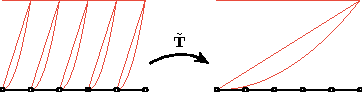
\includegraphics[scale=1.4]{algorithm_4_demo2}
		\caption{The operator $\tilde{\mathbf{T}}$ that maps piecewise polynomials to polynomials on the span $\left[s,e\right]$.}\label{fig:T-tilde}
	\end{subfigure}
	\begin{subfigure}{\linewidth}
		\center
		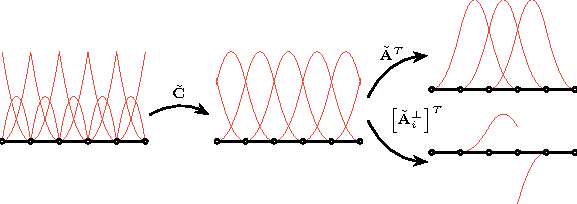
\includegraphics[scale=1.4]{algorithm_4_demo1}
		\caption{The block diagonal matrix $\tilde{\mathbf{C}}$ maps piece Bernstein basis functions to discontinuous B-spline basis functions, the assembly operator $\tilde{\mathbf{A}}$ constructed by restricting the operator $\mathbf{A}$ onto involved elements and spline basis functions maps discontinuous spline basis functions to continuous spline basis functions and the operator $\tilde{\mathbf{A}}^\perp_i$ constructed by restricting the operator $\mathbf{A}^\perp_i$ onto involved elements maps discontinuous spline basis functions to function $\tilde{N}_i$.}\label{fig:C_tilde_and_A_tilde}
	\end{subfigure}
	\caption{Illustration of behaviors of operators in Algorithm.~\ref{alg:modification_weight_new}. }
\end{figure}

The comparison of maximum condition numbers between the matrix $\mathbf{M}$ in Algorithm.~\ref{alg:modification_weight} and the matrix $\mathbf{M}$ in Algorithm.~\ref{alg:modification_weight_new} for constructing $p^\text{th}$ order dual basis function with $p^\text{th}$ order polynomial reproduction ($q=p$) is studied in Figure~\ref{fig:condition_number}. As can be seen, the condition number of $\mathbf{M}$ in Algorithm.~\ref{alg:modification_weight} grows at the rate $p$, whereas the condition number of $\mathbf{M}$ in Algorithm.~\ref{alg:modification_weight_new} is independent of mesh refinements. These results indicate the robustness of Algorithm.~\ref{alg:modification_weight_new}.

\begin{figure}[ht]
	\center
	\includestandalone[scale=1]{dual_basis_condition_number}%     without .tex extension
	% or use \input{mytikz}
	\caption{The growth of the maximum condition numbers of the matrix $\mathbf{M}$ in Algorithm.~\ref{alg:modification_weight} and Algorithm.~\ref{alg:modification_weight_new}.}
	\label{fig:condition_number}
\end{figure}

Thanks to Algorithm.~\ref{alg:modification_weight} and Algorithm.~\ref{alg:modification_weight_new}, the enriched dual basis reproduces polynomial globally (Assumption.~\ref{aspt:global_polynomial_reproduction}), and the construction process guarantees the supported of each enriched dual basis function consists no more than $p+q+1$ elements (Assumption.~\ref{aspt:local_support}). It remains to prove the local stability property (Assumption.~\ref{aspt:local_stability}).

\begin{proof}[Proof of Assumption.~\ref{aspt:local_stability}]
	\begin{align}
		\begin{split}
			\| \quasiid{N}u \|_{H^k(\Omega_e)} &= \| \sum_i \langle {N_i,u} \rangle_{\Omega}\hat{N}_i \|_{H^k(\Omega_e)}\\
			&\leq \| \sum_i \hat{N}_i\|_{H^k(\Omega_e)} \| \langle {\mathbf{N},u} \rangle_{\hat{\Omega}_e} \|_\infty\\
			&= \| \hat{\mathbf{N}}^T\mathbf{1} \|_{H^k(\Omega_e)} \| \langle {\mathbf{N},u} \rangle_{\hat{\Omega}_e} \|_\infty,
		\end{split}
	\end{align}
	where $\mathbf{1}$ is a unit valued vector of the same size as $\hat{\mathbf{N}}$. By rewriting $\hat{\mathbf{N}}$ in its expanded form~\eqref{eq:dual_basis_form}, we have
	\begin{equation}
		\| \quasiid{N}u \|_{H^k(\Omega_e)} \leq  \| \sum_i{B_i} \|_{H^k(\Omega_e)} \| \mathbf{G}^{-T}\mathbf{R}\mathbf{W}\mathbf{1} \|_\infty \| \langle {\mathbf{N},u} \rangle_{\hat{\Omega}_e} \|_\infty.
	\end{equation}
	From the definition of matrix norms, we then have
	\begin{equation}
		\begin{split}
			\| \quasiid{N}u \|_{H^k(\Omega_e)} &\leq \| \sum_i{B_i} \|_{H^k(\Omega_e)} \| \mathbf{G}^{-T}\mathbf{R}\mathbf{W}\|_\infty \| \langle {\mathbf{N},u} \rangle_{\hat{\Omega}_e} \|_\infty\\
			&\leq \| \sum_i{B_i} \|_{H^k(\Omega_e)} \| \mathbf{G}^{-T} \|_\infty \| \mathbf{R} \|_\infty \| \mathbf{W} \|_\infty \| \langle {\mathbf{N},u} \rangle_{\hat{\Omega}_e} \|_\infty.
		\end{split}\label{eq:proof_of_assumption3_1}
	\end{equation}

	Since Bernstein basis forms a partition of unity over each elements, we have that
	\begin{equation}
		\| \sum_i{B_i} \|_{H^k(\Omega_e)} = \| 1 \|_{H^k(\Omega_e)} = \| 1 \|_{L^2(\Omega_e)} = \sqrt{h}.\label{eq:proof_of_assumption3_2}
	\end{equation}

	Let $\mathbf{G}_{\left[ 0,1 \right]}$ be the Gramian matrix defined on the interval $\left[ 0,1 \right]$ and assume $\|\mathbf{G}^{-1}_{\left[ 0,1 \right]}\|_\infty = C_{gi}$, we have
	\begin{equation}
		\| \mathbf{G}^{-T} \|_\infty = \| \mathbf{G}^{-1} \|_\infty = h^{-1} \|\mathbf{G}^{-1}_{\left[ 0,1 \right]}\|_\infty = C_{gi}h^{-1}.\label{eq:proof_of_assumption3_3}
	\end{equation}

	Owing to the fact that the \Bezier element extraction operators are independent of the geometry and are invariant under uniform scaling, their norms are independent of the mesh size. In addition, there are finite number of different \Bezier element extraction operators generated by uniform mesh refinements. Hence, we can assume $\|\mathbf{R}\|_\infty=C_r$. Meanwhile, thanks to Algorithm.~\ref{alg:modification_weight_new}, the construction of $\mathbf{W}$ is geometry and mesh size independent. Hence, we can assume $\|\mathbf{W}\|_\infty=C_w$.\par

	Since spline basis functions are non-negative and also form a partition of unity, from Lemma.~\ref{lemma:local_polynomial_reproduction} and Cauchy-Schwarz inequality, we have that
	\begin{equation}
		\| \langle {\mathbf{N},u} \rangle_{\hat{\Omega}_e} \|_\infty \leq \| \langle {\mathbf{1},u} \rangle_{\hat{\Omega}_e} \|_\infty = \vert \int_{\hat{\Omega}_e} u d\Omega \vert \leq \|1\|_{L^2(\hat{\Omega}_e)} \|u\|_{L^2(\hat{\Omega}_e)}=\sqrt{C_m h} \|u\|_{L^2(\hat{\Omega}_e)}.\label{eq:proof_of_assumption3_4}
	\end{equation}
	where $C_m$ is the number of elements involed in $\hat{\Omega}_e$. By putting Equation~\eqref{eq:proof_of_assumption3_2}, \eqref{eq:proof_of_assumption3_3}, \eqref{eq:proof_of_assumption3_4} into Equation~\eqref{eq:proof_of_assumption3_1}, we have
	\begin{equation}
		\begin{split}
			\| \quasiid{N}u \|_{H^k(\Omega_e)} &\leq C_{gi}C_wC_r \sqrt{C_m} \|u\|_{L^2(\hat{\Omega}_e)} \\
			&\leq C_{gi}C_wC_r\sqrt{C_m}\|u\|_{H^k(\hat{\Omega}_e)}.
		\end{split}
	\end{equation}
	This ends the proof with $C_{st}=C_{gi}C_wC_r\sqrt{C_m}$.
\end{proof}
Hence, the enriched dual basis satisfies all assumptions and will yield optimal approximations.
\FloatBarrier

\section{Applications to $2^\text{nd}$ order and $4^\text{th}$ order mortar isogeometric analysis}\label{sec:dual_mortar}

The enriched dual basis functions can be used to discretize the Lagrange multiplier space for the constructing of constrained finite dimensional space in the dual mortar formulation. In this section, we demonstrate the dual mortar formulations of Poisson problem, linear elasticity problem and biharmonic problem. The formulations are grounded on a two-patch domain (see Figure~\ref{fig:two_patch_domain}) and the extension to multiple-patch domains is straightforward.

\begin{figure}[ht]
	\center
	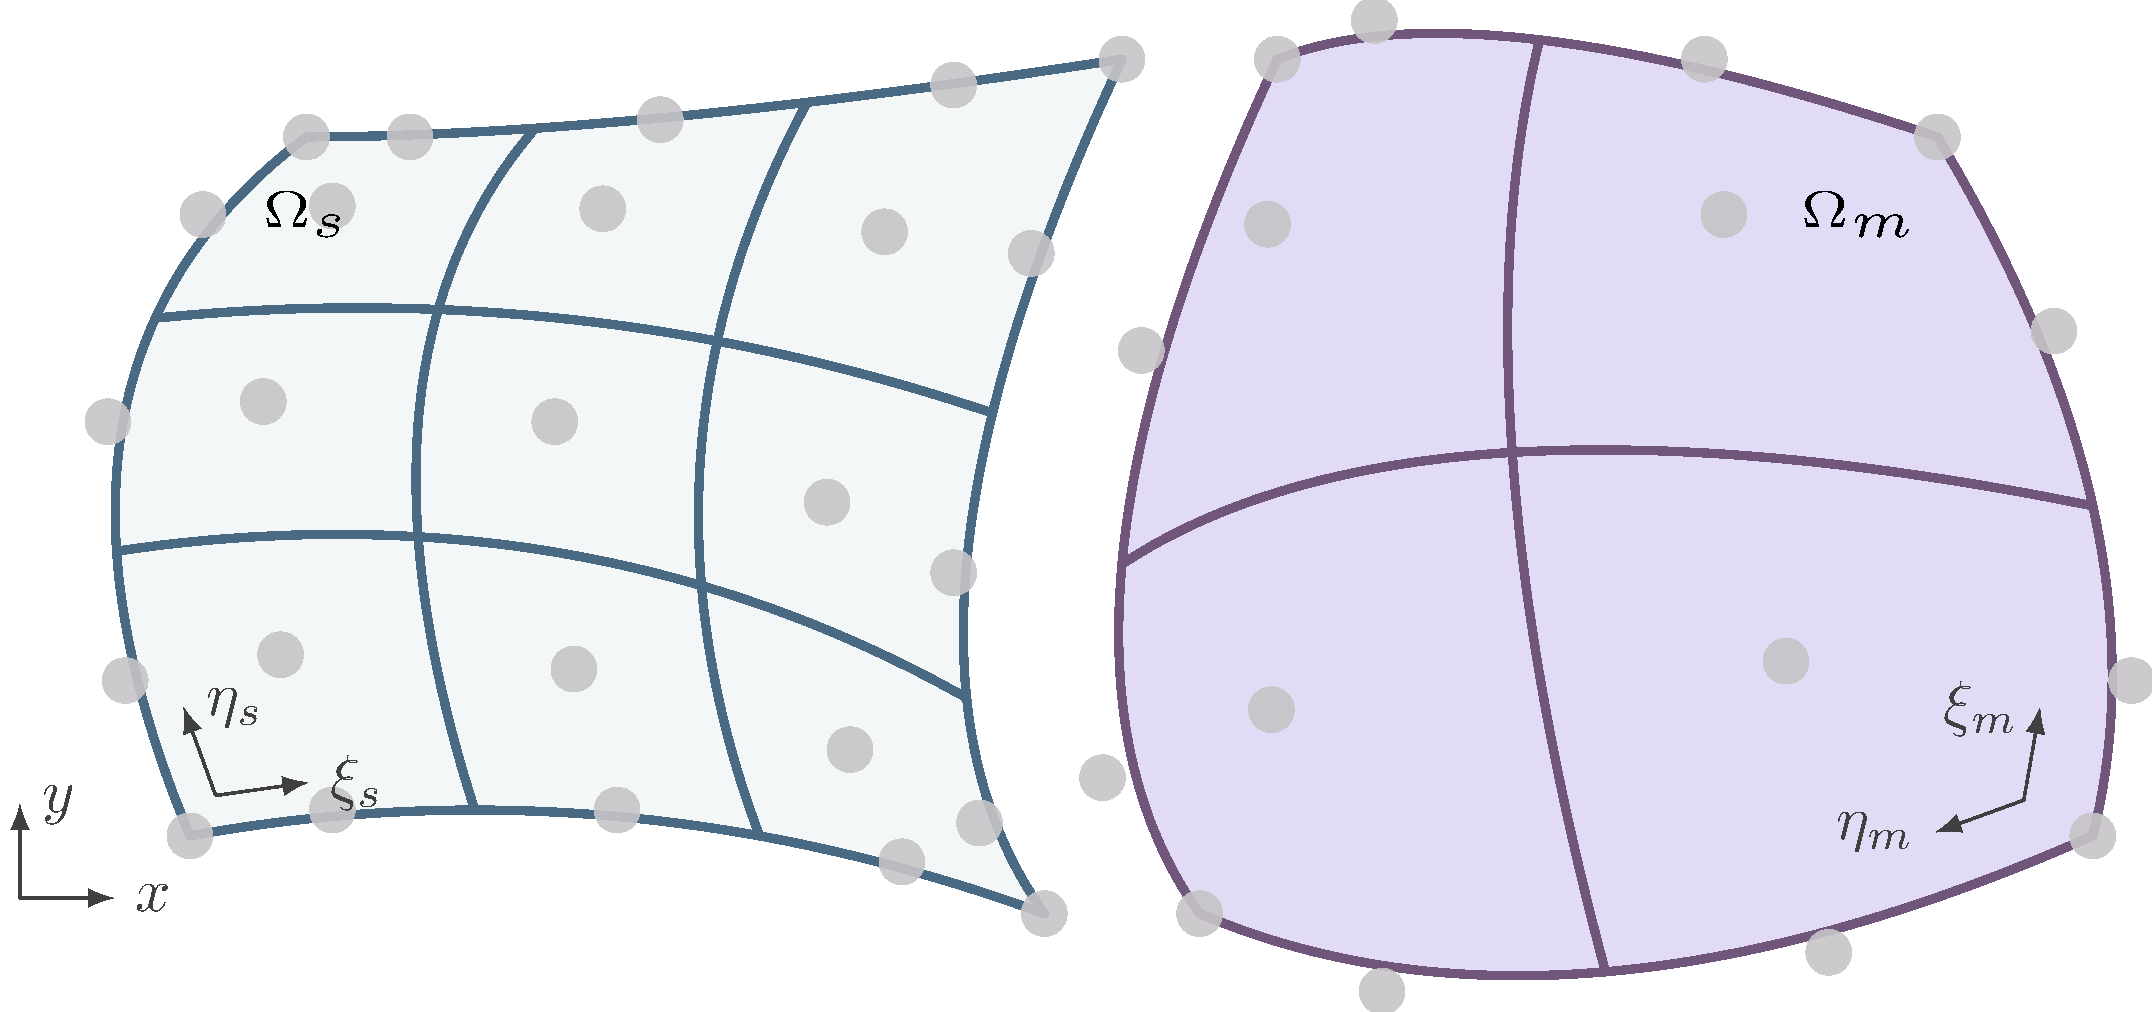
\includegraphics[width=.7\columnwidth]{two_patch_domain}
	\caption{A two-patch planar domain $\Omega$ consisting of two patches $\Omega_s$ and $\Omega_m$. }\label{fig:two_patch_domain}
\end{figure}

\subsection{Vertex modification}

For a multi-patch decomposition, at least three patches meet at an interior vertex and several interfaces can share this vertex as a common endpoint. If we still discretize the Lagrange multiplier space with the same dimension as univariate basis of the slave side, we obtain too many constraints. Some of the control points in the neighborhood of a vertex may serve as both slave nodes and master nodes. As a result, the matrix $\mathbf{B}^\perp$ cannot be formed elegantly as Equation~\eqref{iii-eq:null-space}. In addition, it has been demonstrated in Chapter~\ref{chp:chapter3} that, such $\mathcal{V}^h$ constructed by global dual basis does not satisfy the \textit{inf-sup} condition, leading to a sub-optimal approximation error. Hence, vertex modifications are needed to relax overly constrained linear system.\par

In general, the vertex modification can be achieved by reducing the dimension of the Lagrange multiplier space. For second order problems, a Lagrange multiplier space of codimension $2$ of the trace space of the slave side is sufficient to remove redundant constraints; whereas, for fourth order problems, a Lagrange multiplier space of codimension $4$
of the trace space of the slave side is prefered. To construct an enriched dual basis of codimension $2c$, we remove the first $c$ and the last $c$ vectors in $\{\mathbf{A}_i\}_{i=0}^{n_N-1}$, leaving $\{\mathbf{A}_i\}_{i=c}^{n_N-1-c}$ a $n_N-2c$ dimensional vector space. The orthonormal vector basis of the null space of $\spn\{\mathbf{A}_i\}_{i=c}^{n_N-1-c}$ can be written as $\{\mathbf{A}^\perp_i\}_{i=0}^{n_B-n_N-1}\bigcup\{\mathbf{A}^n_i\}_{i=0}^{c-1}\bigcup\{\mathbf{A}^n_i\}_{i=n_N-c}^{n_N-1}$. Now, we can construct $\mathbf{W}^\text{ini}$ from $\{\mathbf{A}_i\}_{i=c}^{n_N-1-c}$ via Equation~\eqref{eq:initial_guess} and assemble $\mathbf{W}^\text{mod}$ from $\{\mathbf{A}^\perp_i\}_{i=0}^{n_B-n_N-1}\bigcup\{\mathbf{A}^n_i\}_{i=0}^{c-1}\bigcup\{\mathbf{A}^n_i\}_{i=n_N-c}^{n_N-1}$ via Algorithm.~\ref{alg:modification_weight_new}. The resulted dual basis is $2c$ dimensional less than the original basis and satisfies the global idempotence.

\subsection{Domain decomposition for $2^\text{nd}$ order problems}

Due to the existence of the first order weak derivative in the weak form of $2^\text{nd}$ order problems, the constrained space $\mathcal{V}^h$ should weakly satisfy $C^0$ continuity constraint across the interface $\Gamma$. Hence, the constrained space $\mathcal{V}^h$ for $2^\text{nd}$ order problems is given by

\begin{equation}
	\mathcal{V}^h\coloneqq \left\{ v\in \mathcal{X}^h \left|\quad \int_{\Gamma} \mu \left[ u \right] d \Gamma=0,\quad \forall \mu\in \mathcal{M}^h \right. \right\},
\end{equation}
where the Lagrange multiplier space $\mathcal{M}^h$ is two dimension less than the trace space of the slave side. As a result, in addition to the interface nodes of the master side, the first and the last interface nodes of the slave side also serve as master nodes (see Figure~\ref{fig:2nd_order_nodes}). 
\begin{figure}[ht]
	\center
	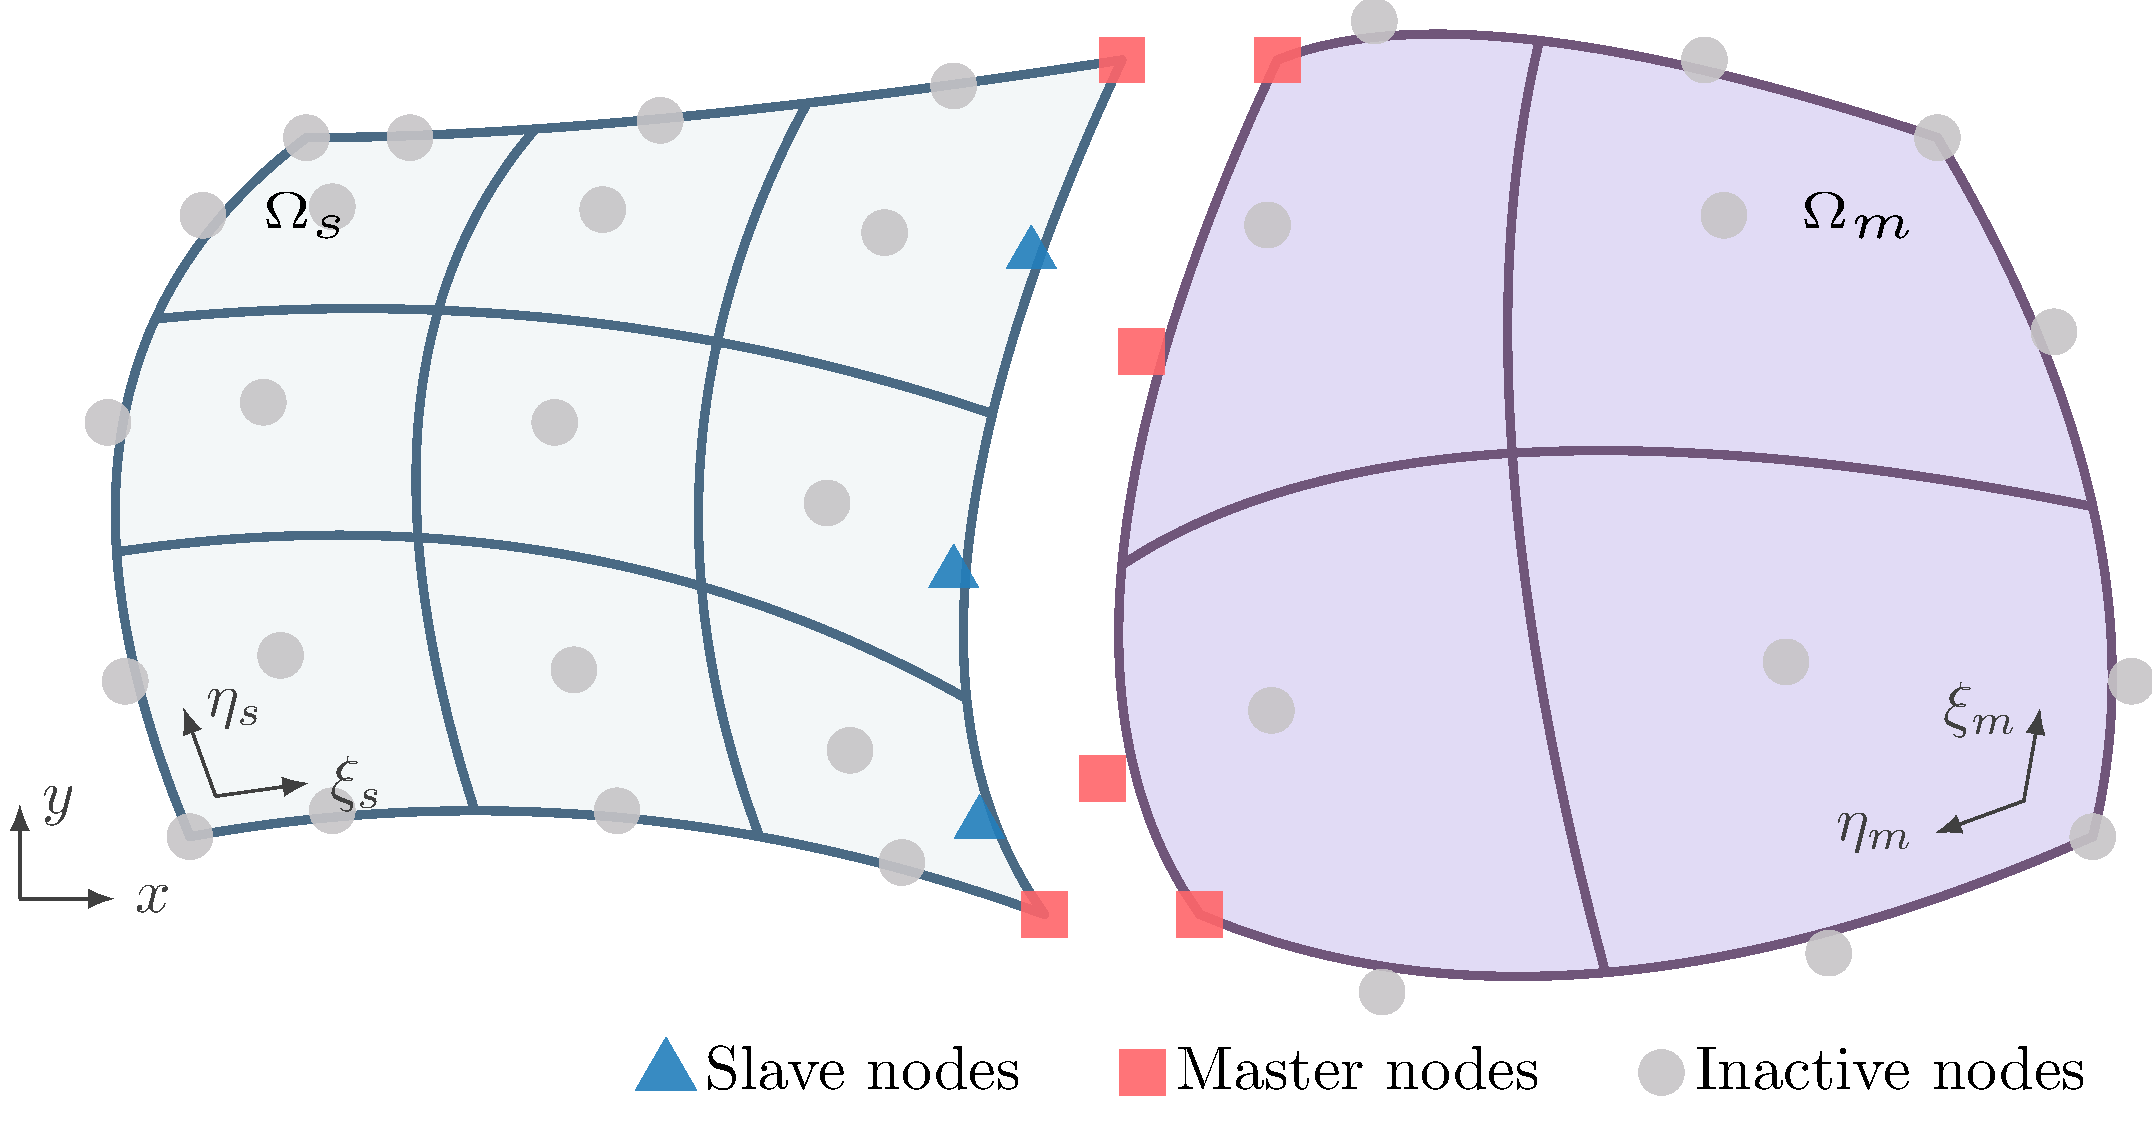
\includegraphics[width=.7\columnwidth]{two_patch_domain_poisson}
	\caption{The classification of nodes on the intersection for $2^\text{nd}$ order problems. }\label{fig:2nd_order_nodes}
\end{figure}

\subsection{Domain decomposition for $4^\text{th}$ order problems}

Due to the existence of the second order weak derivative in the weak form of $4^\text{nd}$ order problems, the constrained space $\mathcal{V}^h$ should weakly satisfy $C^1$ continuity constraint across the interface $\Gamma$. Hence, two Lagrange multiplier are needed to apply $C^0$ continuity constraint and $C^1$ continuity constraint, correspondingly. The constrained space $\mathcal{V}^h$ for $4^\text{nd}$ order problems is given by

\begin{equation}
	\mathcal{V}^h\coloneqq \left\{ v\in \mathcal{X}^h \left| \quad  \left\{\begin{alignedat}{2}
		&\int_{\Gamma} \mu_0 \left[ u \right] d \Gamma=0, &&\forall \mu_0\in \mathcal{M}_0^h\\
		&\int_{\Gamma} \mu_1 \left[ \frac{\partial u}{ \partial \xi_s} \right] d \Gamma=0\text{ if }\Gamma\parallel\eta_s\text{ or }\int_{\Gamma} \mu_1 \left[ \frac{\partial u}{ \partial \eta_s} \right] d\Gamma=0\text{ if }\Gamma\parallel\xi_s,\quad&&\forall\mu_1\in \mathcal{M}_1^h
	\end{alignedat}\right. \right. \right\},
\end{equation}
where both $\mathcal{M}_0^h$ and $\mathcal{M}_1^h$ are $4$ dimension less than the trace space of the slave side. As a result, four nodes in the neighborhood of each vertices of $\Omega_s$ are classified as master nodes.

\begin{figure}[ht]
	\center
	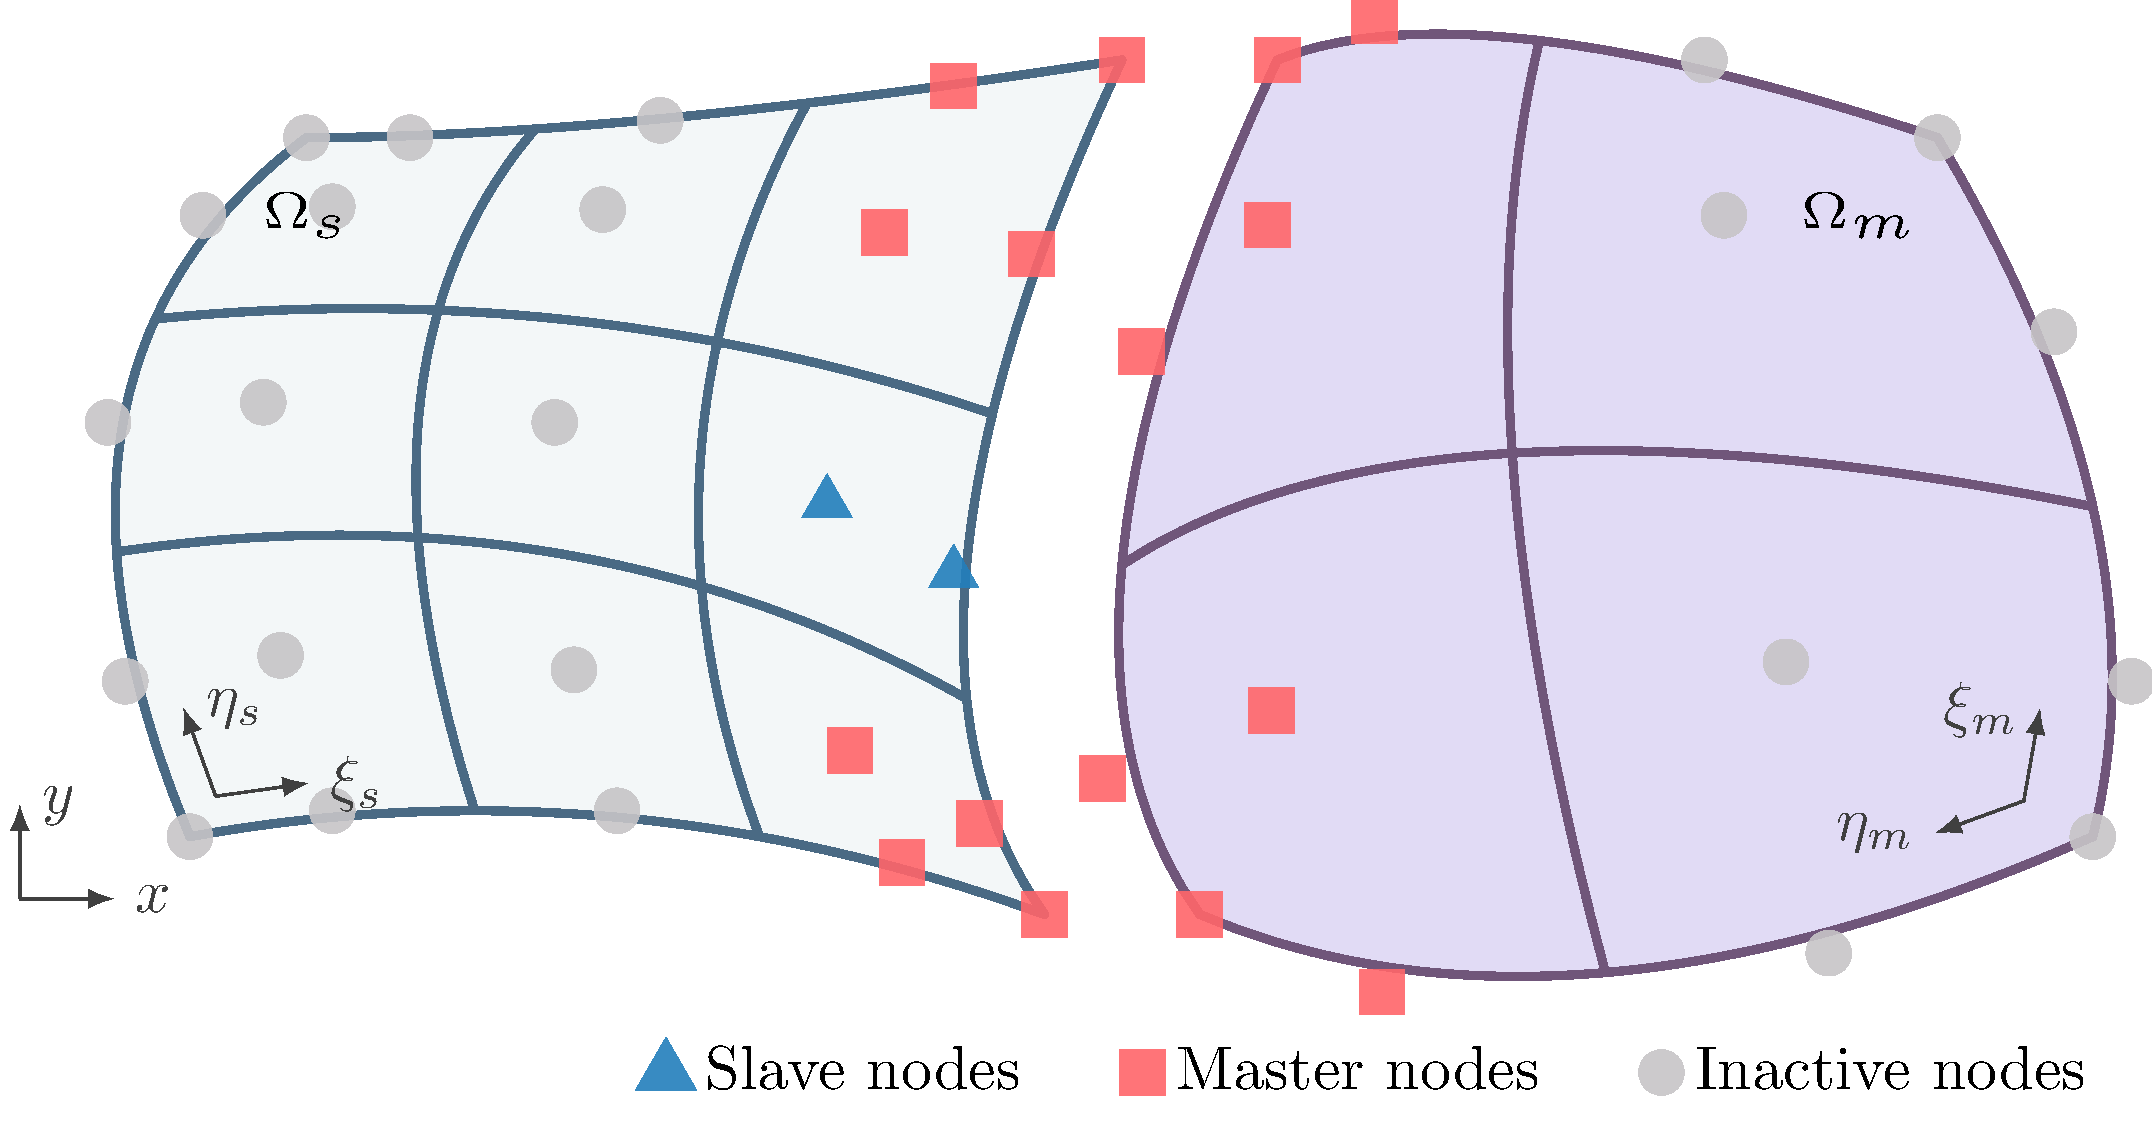
\includegraphics[width=.7\columnwidth]{two_patch_domain_biharmonic}
	\caption{The classification of nodes on the intersection for biharmonic problems ($4^\text{th}$ order problems). }
\end{figure}

\FloatBarrier

\section{Numerical examples}\label{sec:examples}

In this section, we investigate the performance of the enriched dual basis in several challenging $2^\text{nd}$ and $4^\text{th}$ order benchmarks. The first example is a Poisson's problem over a four-patch square domain, where the intersections are all non-matching parameterized. In the second problem, we model an infinite plate with a hole by four non-conforming NURBS patches. The third benchmark is a biharmonic over a five-patch square domain. A simply supported square Kirchhoff-Love plate is tested as our fourth example. To verify the robustness of enriched dual basis and dual mortar formulation for $4^\text{th}$ order problems, we consider the Cahn-Hilliard equation as the last benchmark. All numerical problem are solved by the Eigen library~\cite{eigenweb}. Due to the asymmetric structure of the consistency tangent matrix in Cahn-Hilliard problem, the BiCGSTAB solver is used whereas the conjugate gradient solver is used for the rest of problems. Note that extraordinary points are presented in all tested topologies. For the \Bezier dual basis, we adopt the extraordinary modification utilized in Chapter~\ref{chp:chapter3}.\par

Results obtained from the enriched dual basis are denoted by Enrich-$Q_i$. As a comparison, the performances of the enriched dual basis are compared with the global dual basis (labeled by $L^2$-$Q_i$) and the \Bezier dual basis (labeled by \Bezier-$Q_i$). For all $2^\text{nd}$ order problems, the polynomial reproduction order $q$ is set to $p-1$ for the construction of the $p^\text{th}$ order enriched dual basis whereas $q=p-2$ for all $4^\text{th}$ order problems. This setting ensures the sparsest stiffness matrix while maintains the optimality. All enriched dual basis are constructed via Algorithm.~\ref{alg:modification_weight_new}.

\subsection{Poisson problem}\label{sec:poisson_problem}

We start by solving the Poisson's equation $-\Delta u=f$ over the domain $\left[ 0, 1\right]\times \left[ 0, 1\right]$. The domain is decomposed into four patches, shown in Figure.~\ref{fig:Poisson_mesh}. The manufactured solution is given as:
\begin{equation}
	u(x,y) = \sin(2\pi x)\sin(2 \pi y).
\end{equation}
This manufactured solution satisfies the homogeneous Dirichlet boundary condition ($u=0$) and is demonstrated in Figure.~\ref{fig:Poisson_manufacture}.

\begin{figure}[ht]
	\center
	\begin{subfigure}[t]{.45\linewidth}
		\center
		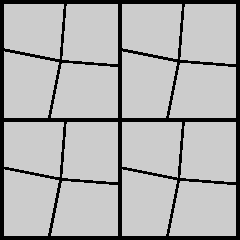
\includegraphics[scale=1.35]{four_patches_nonconform_nonmatch}
		\caption{Non-matching parameterized non-conforming four-patch mesh}\label{fig:Poisson_mesh}
	\end{subfigure}
	\begin{subfigure}[t]{.45\linewidth}
		\center
		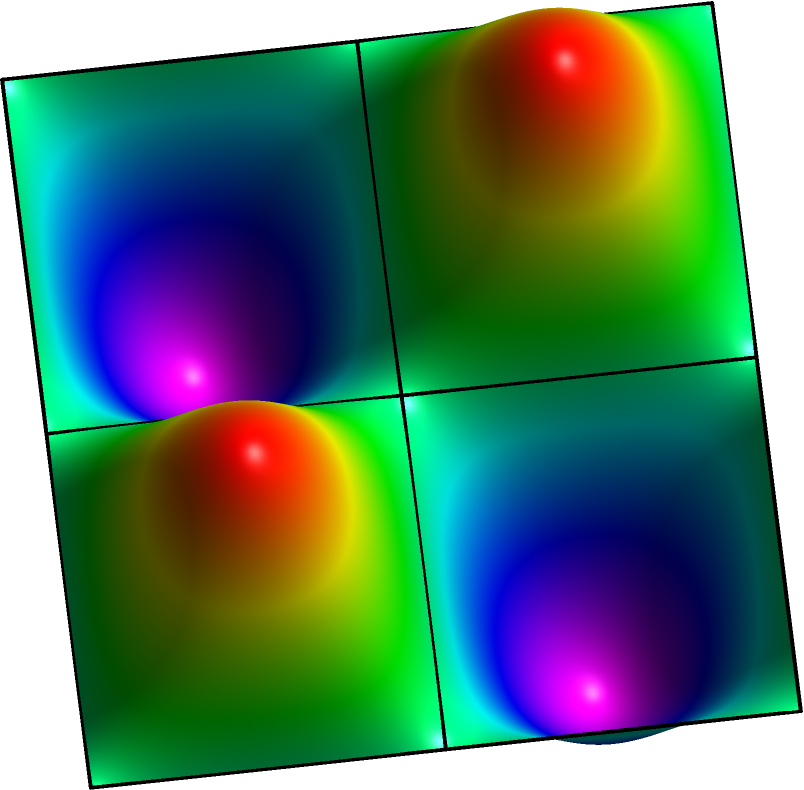
\includegraphics[scale=.41]{four_patches_solution-plot}
		\caption{The manufactured solution}\label{fig:Poisson_manufacture}
	\end{subfigure}
	\caption{The decomposition and discretization of the domain $\Omega=\left[ 0, 1\right]\times \left[ 0, 1\right]$ and the manufactured solution that satisfies $u=0$ on $\partial\Omega$, which are utilized as the initial mesh and the reference solution in Section~\ref{sec:poisson_problem}.}
\end{figure}

Convergence plots in $L^2$ norm and $H^1$ norm are shown in Figure.~\ref{fig:Poisson_convergence}. We observe optimal convergence of the enriched dual basis in all tested polynomial orders ($p=\left\{2,3,\dots,5\right\}$) in both measures. For $p=2,3$, the errors of the enriched dual basis are close to that of the global dual basis, whereas uniform shifts have been observed from the enriched dual basis of $p=4,5$. We speculate that the cause of vertical shifts of error curves is the non-matching parameterization. Since the enriched dual basis functions enjoy larger support size, the size of an extension element $\hat{\Omega}_e$ of the enriched dual basis will be significantly larger than that of the standard B-spline basis. As a result, the local estimation error of the enriched dual basis will be larger than that of the standard B-spline basis. And the irregular parameterization seems to aggravate this effect. Regardless of the slightly shift, however, the optimal convergence rates have been observed in both measures. The \Bezier dual basis, as expected, demonstrates sub-optimal convergence in both $L^2$ and $H^1$ for $p=3,4,5$. In addition, in the asymptotical region, the error increases as the polynomial order is increased.\par

\begin{figure}[ht]
	\center
	\captionsetup[subfigure]{labelformat=empty}
	\begin{subfigure}{.45\linewidth}
		\center
		\includestandalone[scale=.8]{four_patch_poisson_L2}
	\end{subfigure}\hspace{2mm}
	\begin{subfigure}{.45\linewidth}
		\center
		\includestandalone[scale=.8]{four_patch_poisson_H1}
	\end{subfigure}
	\caption{Convergence plots for non-matching parameterized non-conforming patch coupling in Section~\ref{sec:poisson_problem}. Left: error measured in $L^2$ norm. Right: error measured in $H^1$ norm.}\label{fig:Poisson_convergence}
\end{figure}

Contour plots of $\text{err} = u-u^h$ for cubic mesh after three refinements are shown in Figure.~\ref{fig:contour_Poisson}. As can be seen, the contour plot of the enriched dual basis is similar to that of the global dual basis, except some spikes in the neighbourhood of extraordinary points. On the other hand, a significant amount of oscillation is observed for the \Bezier dual basis along each intersection. It is deserved to notice that the in-domain error (approximation error) remains in the similar level as the other two cases.

\begin{figure}[ht]
	\center
	\captionsetup[subfigure]{labelformat=empty}
	\begin{subfigure}[t]{.45\linewidth}
		\center
		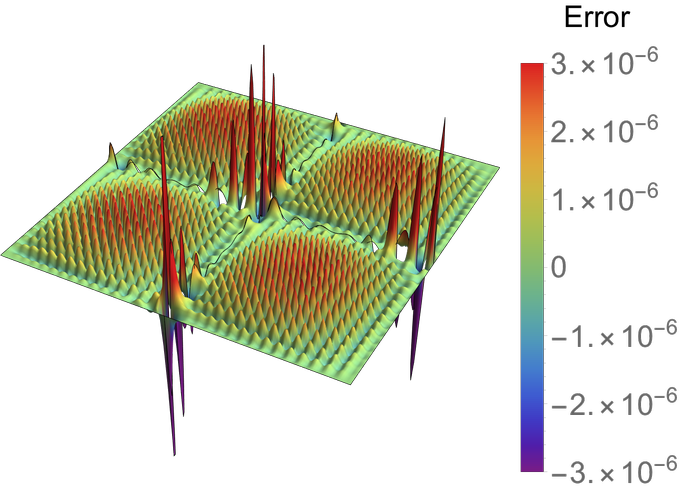
\includegraphics[scale=.52]{four_patch_poisson_op_contour}
		\caption{Enrich-$Q_3$}
	\end{subfigure}
	\begin{subfigure}[t]{.45\linewidth}
		\center
		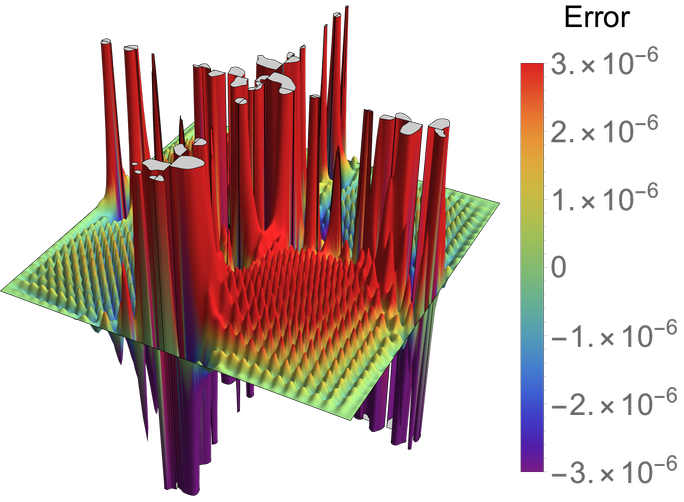
\includegraphics[scale=.52]{four_patch_poisson_Bezier_contour}
		\caption{\Bezier-$Q_3$}
	\end{subfigure}\\
	\center
	\begin{subfigure}[t]{.45\linewidth}
		\center
		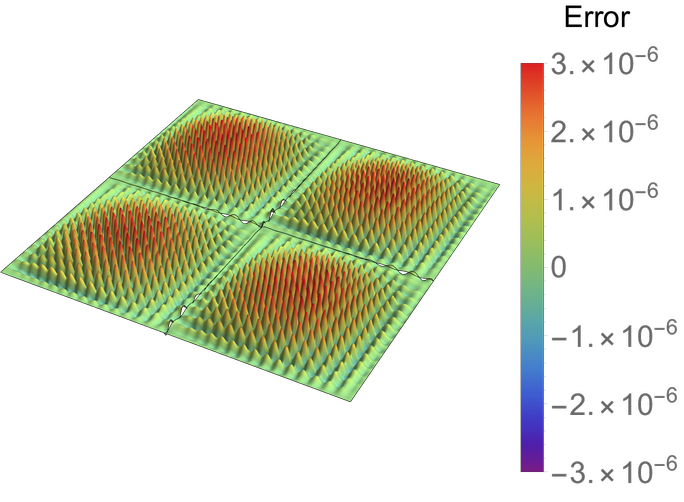
\includegraphics[scale=.52]{four_patch_poisson_L2_contour}
		\caption{$L^2$-$Q_3$}
	\end{subfigure}
	\caption{Contour plots of $\text{err} =u-u^h$ for the Poisson problem on the four-patch domain ($p=3$, and the mesh is obtained after three refinements). }\label{fig:contour_Poisson}
\end{figure}

\subsection{Linear elasticity -- plate with a hole}\label{sec:plate_with_a_hole}

To test the performance of the enriched dual basis over vector fields, we consider a linear elastic problem. The problem setup and the multi-patch discretization are demonstrated in Figure.~\ref{fig:plate_with_hole_setup}.  The traction along the outer edge is evaluated from the exact solution which is given by

\begin{align}
	\begin{split}
		\sigma_{rr}(r,\theta)&=\dfrac{T_x}{2}(1-\dfrac{R_1^2}{r^2})+\dfrac{T_x}{2}(1-4\dfrac{R_1^2}{r^2}+3\dfrac{R_1^4}{r^4})\cos(2\theta),\\
		\sigma_{\theta\theta}(r,\theta)&=\dfrac{T_x}{2}(1+\dfrac{R_1^2}{r^2})-\dfrac{T_x}{2}(1+3\dfrac{R_1^4}{r^4})\cos(2\theta),\\
		\sigma_{r\theta}(r,\theta)&=-\dfrac{T_x}{2}(1+2\dfrac{R_1^2}{r^2}-3\dfrac{R_1^4}{r^4})\sin(2\theta).
	\end{split}
\end{align}

\begin{figure}[ht]
	\captionsetup[subfigure]{width=0.9\textwidth}
	\center
	\begin{subfigure}[t]{.3\textwidth}
		\center
		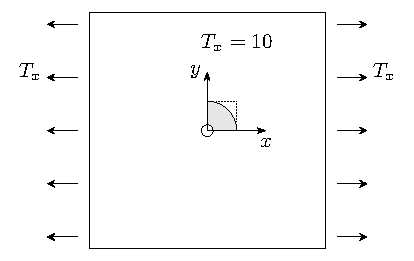
\includegraphics[scale=.7]{Platewithhole}
		\caption{Infinite plate with a hole subjected to uniaxial tension at $x=\pm \infty$}
	\end{subfigure}
	\begin{subfigure}[t]{.3\textwidth}
		\center
		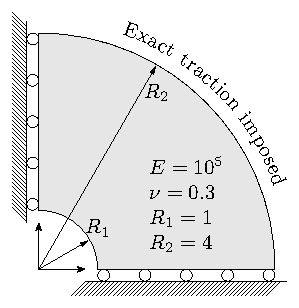
\includegraphics[scale=.7]{annular}
		\caption{The computational geometry, boundary conditions and material parameters. }
	\end{subfigure}
	\begin{subfigure}[t]{.3\textwidth}
		\center
		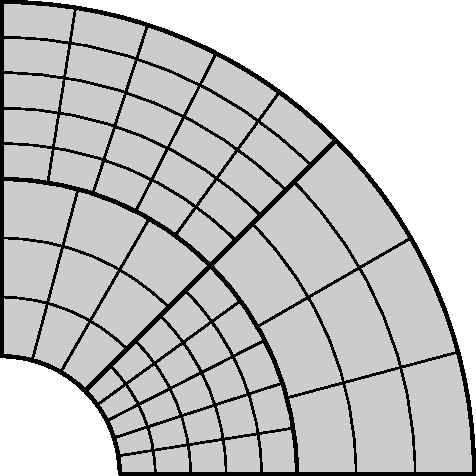
\includegraphics[scale=.45]{annular_mesh}
		\caption{The non-conforming four-patch mesh}
	\end{subfigure}
	\caption{The decomposition and discretization of the domain $\Omega$ and the manufactured solution that satisfies $u=0$ on $\partial\Omega$, which are utilized as the initial mesh and the reference solution in Section~\ref{sec:plate_with_a_hole}.}\label{fig:plate_with_hole_setup}
\end{figure}

The relative error of $\mathbf{u}$ are mesured in $L^2$ norm and energy semi-norm:
\begin{equation}
	\|\mathbf{u}-\mathbf{u}^h\|_{E}:=\sum_k\int_{\Omega_k}\frac{1}{2}\mathbf{\sigma}(\mathbf{u}-\mathbf{u}^h) \colon \mathbf{\epsilon}(\mathbf{u}-\mathbf{u}^h) d \Omega.
\end{equation}
Convergence plots for both measures are given in Figure.~\ref{fig:convergence_plate_with_hole}. Similar to the scalar problem, both the enriched dual basis and the global dual basis yield optimal convergence results for all tested polynomial orders in both measures. In addition, due to the absence of non-matching parameterized intersections, the convergence plots of the enriched dual basis are all identical to that of the global dual basis. The
convergence plots of the\Bezier dual basis, again, demonstrate sub-optimal performances.\par

\begin{figure}[ht]
	\center
	\captionsetup[subfigure]{labelformat=empty}
	\begin{subfigure}{.45\linewidth}
		\center
		\includestandalone[scale=.8]{four_patch_elasticity_L2}
	\end{subfigure}\hspace{2mm}
	\begin{subfigure}{.45\linewidth}
		\center
		\includestandalone[scale=.8]{four_patch_elasticity_energy}
	\end{subfigure}
	\caption{Convergence plots for simple non-conforming patch coupling in Section~\ref{sec:plate_with_a_hole}. Left: error measured in $L^2$ norm. Right: error measured in energy semi-norm.}\label{fig:convergence_plate_with_hole}
\end{figure}

Contour plots of $\text{err} = u_x - u_x^h$ at $p=3$ after three refinements are shown in Figure.~\ref{fig:contour_plate_with_hole}. As can be seen, the contour plots of both the enriched dual basis and the global dual basis are the same. The \Bezier dual basis, however, yields tremendous oscillation along each intersections. Again, the errors in each patch are in the similar level as for the global dual basis, which confirms that the main contribution of the sub-optimality is the consistency error.

\begin{figure}[ht]
	\center
	\captionsetup[subfigure]{labelformat=empty}
	\begin{subfigure}[t]{.45\linewidth}
		\center
		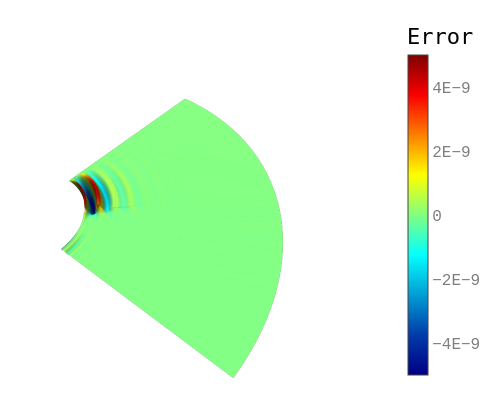
\includegraphics[scale=.4]{op_annular}
		\caption{Enrich-$Q_3$}
	\end{subfigure}
	\begin{subfigure}[t]{.45\linewidth}
		\center
		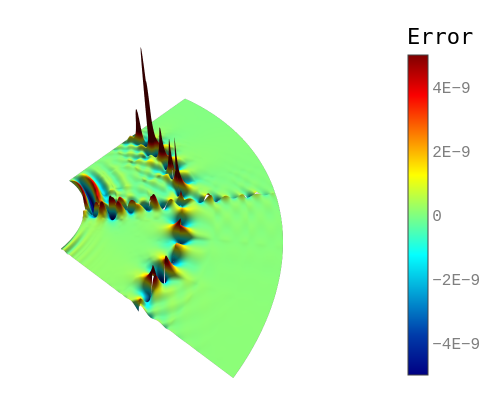
\includegraphics[scale=.4]{bezier_annular}
		\caption{\Bezier-$Q_3$}
	\end{subfigure}\\
	\center
	\begin{subfigure}[t]{.45\linewidth}
		\center
		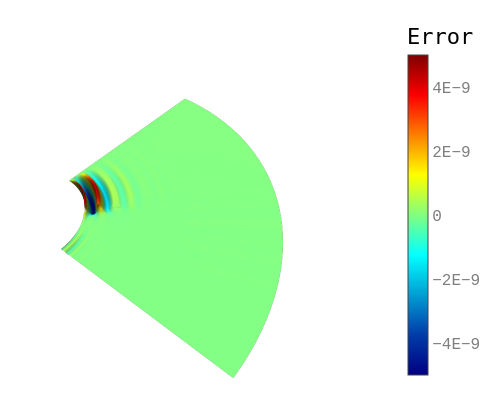
\includegraphics[scale=.4]{l2_annular}
		\caption{$L^2$-$Q_3$}
	\end{subfigure}
	\caption{Contour plots of $\text{err} = u_x-u^h_x$ for the linear elastic problem on the four-patch domain ($p=3$, and the mesh is obtained after three refinements). }\label{fig:contour_plate_with_hole}
\end{figure}
\FloatBarrier

\subsection{Biharmonic problem}\label{sec:biharmonic_problem}

We next consider a homogeneous biharmonic problem over the domain $\left[0, 1\right]\times \left[0, 1\right]$, with the manufactured solution
\begin{equation}
	u(x,y)=\sin(2\pi{x})^2\sin(2\pi{y})^2.
\end{equation}
The discretization and the manufactured solution are depicted in Figure.~\ref{fig:biharmonic_mesh}.
\begin{figure}[ht]
	\center
	\begin{subfigure}[t]{.45\linewidth}
		\center
		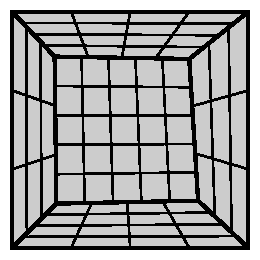
\includegraphics[scale=1.35]{five_patches_mesh}
		\caption{Non-conforming five-patch mesh}
	\end{subfigure}
	\begin{subfigure}[t]{.45\linewidth}
		\center
		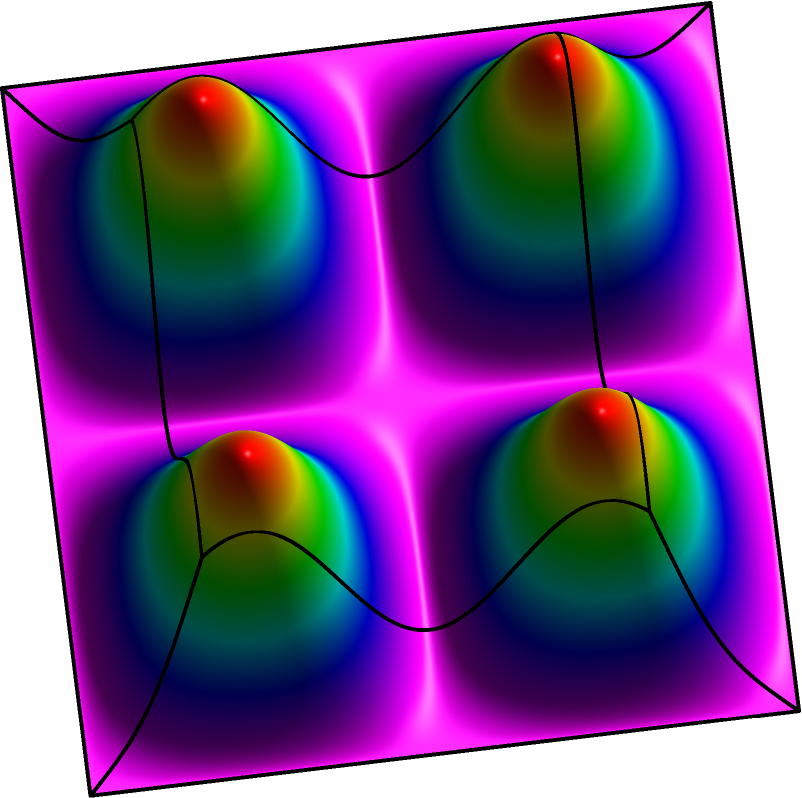
\includegraphics[scale=.425]{five_patch_solution-plot}
		\caption{The manufactured solution}
	\end{subfigure}
	\caption{The decomposition and discretization of the domain $\Omega$ and the manufactured solution that satisfies $u=\frac{\partial u}{\partial \mathbf{n}}=0$ on $\partial\Omega$, which are utilized as the initial mesh and the reference solution in Section~\ref{sec:biharmonic_problem}.}\label{fig:biharmonic_mesh}
\end{figure}

Convergence plots for the biharmonic benchmark are shown in Figure.~\ref{fig:convergence_biharmonic}. The enriched dual basis with $q=p-2$ generates optimal results for $p=2,3,4$ and the convergence plots are identical to that of the global dual basis. Note that the optimal convergence rate for quadratic basis functions is $\mathcal{O}(h^2)$ in $L^2$ norm for biharmonic problems. For the case of $p=5$, we observe sub-optimal convergence for both the enriched dual basis and the global dual basis at the last refinement in $L^2$ norm. However, no sub-optimality has been observed in $H^2$ norm. This phenomenon indicates that the error happens at certain digits of the floating point vector $\mathbf{U}^\text{mortar}$ (between $7^\text{th}$ and $10^\text{th}$ digit for this case). We infer that the cause of the sub-optimality is the conditioning of the stiffness matrix. In addition, studies~\cite{li2008effective} show that the growth rate of condition number for biharmonic problem is $\mathcal{O}(-h^4)$, which is huge, compared with $\mathcal{O}(-h^2)$ for Poisson's problem by finite element method. This explains why ill-conditioning of biharmonic problem happens much earlier than that of Poisson's problem. We also attribute the slightly better performance of the enriched dual basis functions to their compact support and the robust construction algorithm (Algorithm.~\ref{alg:modification_weight_new}). Again, the \Bezier dual basis leads to sub-optimal behavior for higher order elements.\par

\begin{figure}[ht]
	\center
	\captionsetup[subfigure]{labelformat=empty}
	\begin{subfigure}{.45\textwidth}
		\center
		\includestandalone[scale=.8]{five_patch_biharmonic_L2}
	\end{subfigure}\hspace{2mm}
	\begin{subfigure}{.45\textwidth}
		\center
		\includestandalone[scale=.8]{five_patch_biharmonic_H2}
	\end{subfigure}
	\caption{Convergence plots for five non-conforming patch coupling in Section~\ref{sec:biharmonic_problem}. Left: error measured in $L^2$ norm. Right: error measured in $H^2$ norm.}\label{fig:convergence_biharmonic}
\end{figure}

Contour plots for cubic mesh after two refinements are given in Figure.~\ref{fig:contour_biharmonic}. Similar to $2^\text{nd}$ order problems, the contour plot of the enriched dual basis is identical to that of the global dual basis, as the result of the absence of non-matching parameterized interfaces. However, due to the involving of control points that are one column away from the intersection, the consistency error of the \Bezier dual bais case penetrates into each patches for a relatively rough mesh.

\begin{figure}[ht]
	\center
	\captionsetup[subfigure]{labelformat=empty}
	\begin{subfigure}[t]{.45\linewidth}
		\center
		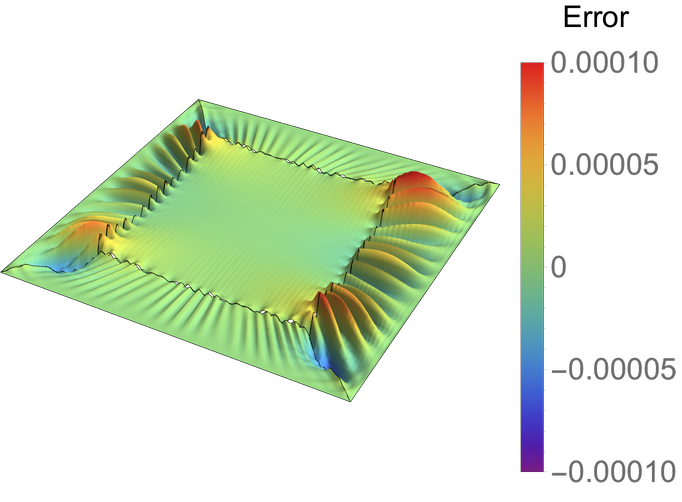
\includegraphics[scale=.52]{five_patch_biharmonic_op_contour}
		\caption{Prop-$Q_3$}
	\end{subfigure}
	\begin{subfigure}[t]{.45\linewidth}
		\center
		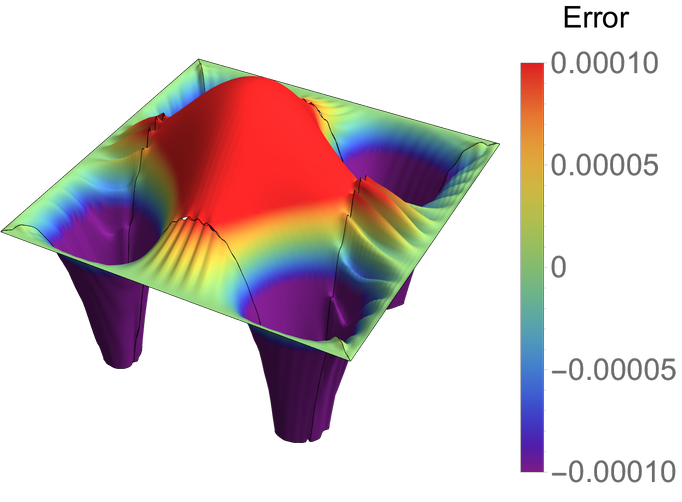
\includegraphics[scale=.52]{five_patch_biharmonic_Bezier_contour}
		\caption{\Bezier-$Q_3$}
	\end{subfigure}\\
	\center
	\begin{subfigure}[t]{.45\linewidth}
		\center
		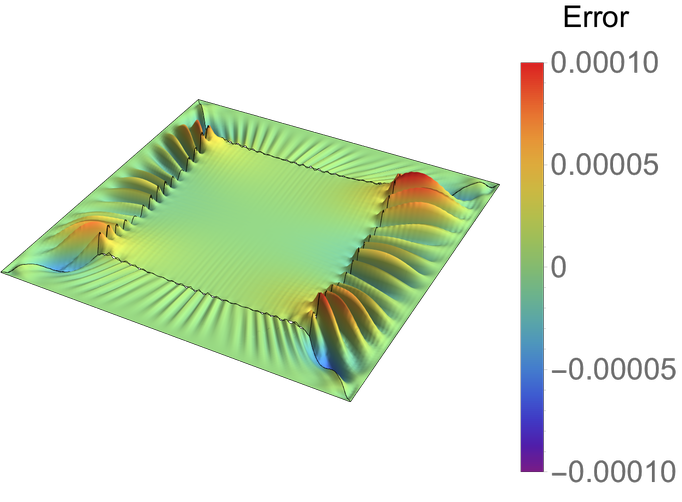
\includegraphics[scale=.52]{five_patch_biharmonic_L2_contour}
		\caption{$L^2$-$Q_3$}
	\end{subfigure}
	\caption{Contour plots of $\text{err}=u-u^h$ for the biharmonic problem on the five-patch domain ($p=3$, and the mesh is obtained after two refinements). }\label{fig:contour_biharmonic}
\end{figure}


\subsection{Kirchhoff plate}\label{sec:kl-plate_problem}

The last benchmark with analytical solution is a simply supported square Kirchhoff plate. The bending moments of Kirchhoff plate is given by:
\begin{equation}
	\begin{split}
		M_{xx} &= -D\left( \frac{\partial^2 w}{\partial x^2} + \nu \frac{\partial^2 w}{\partial y^2}\right),\\
		M_{yy} &= -D\left( \frac{\partial^2 w}{\partial y^2} + \nu \frac{\partial^2 w}{\partial x^2}\right),\\
		M_{xy} &= -D(1-\nu) \frac{\partial^2 w}{\partial xy},
	\end{split}
\end{equation}
where $w$ is the vertical displacement, $D = \frac{Et^3}{12(1-\nu^2)}$, $t$ is the thickness, $E$ is the Young's modulus and $\nu$ is the Poisson's ratio. The governing equation of Kirchhoff plate can be derived as
\begin{equation}
	\frac{\partial^4 w}{\partial x^4} + \frac{\partial^4 w}{\partial x^2y^2} + \frac{\partial^4 w}{\partial y^4} = \frac{q}{D}
\end{equation}
where $q$ is the pressure. In this benchmark, we consider a square plate with $L=12$ subjected to a sinusoidal presure load of
\begin{equation}
	q(x,y) = -\sin(\frac{\pi x}{L}) \sin(\frac{\pi y}{L}).
\end{equation}
We also adopt $t=0.375$, $E=4.8\times 10^5$ and $\nu = 0.38$. The analytical solution is given by
\begin{equation}
	w(x, y) = -\frac{L^4}{4D\pi^4}\sin(\frac{\pi x}{L}) \sin(\frac{\pi y}{L}).
\end{equation}
The geometry, discretization and the analytical solution of vertical displacement are shown in Figure.~\ref{fig:kirchhoff_mesh}. Note that the green intersection is non-matching parameterized, whereas red curves are coupled non-comformingly. \par

\begin{figure}[ht]
	\center
	\begin{subfigure}[t]{.45\linewidth}
		\center
		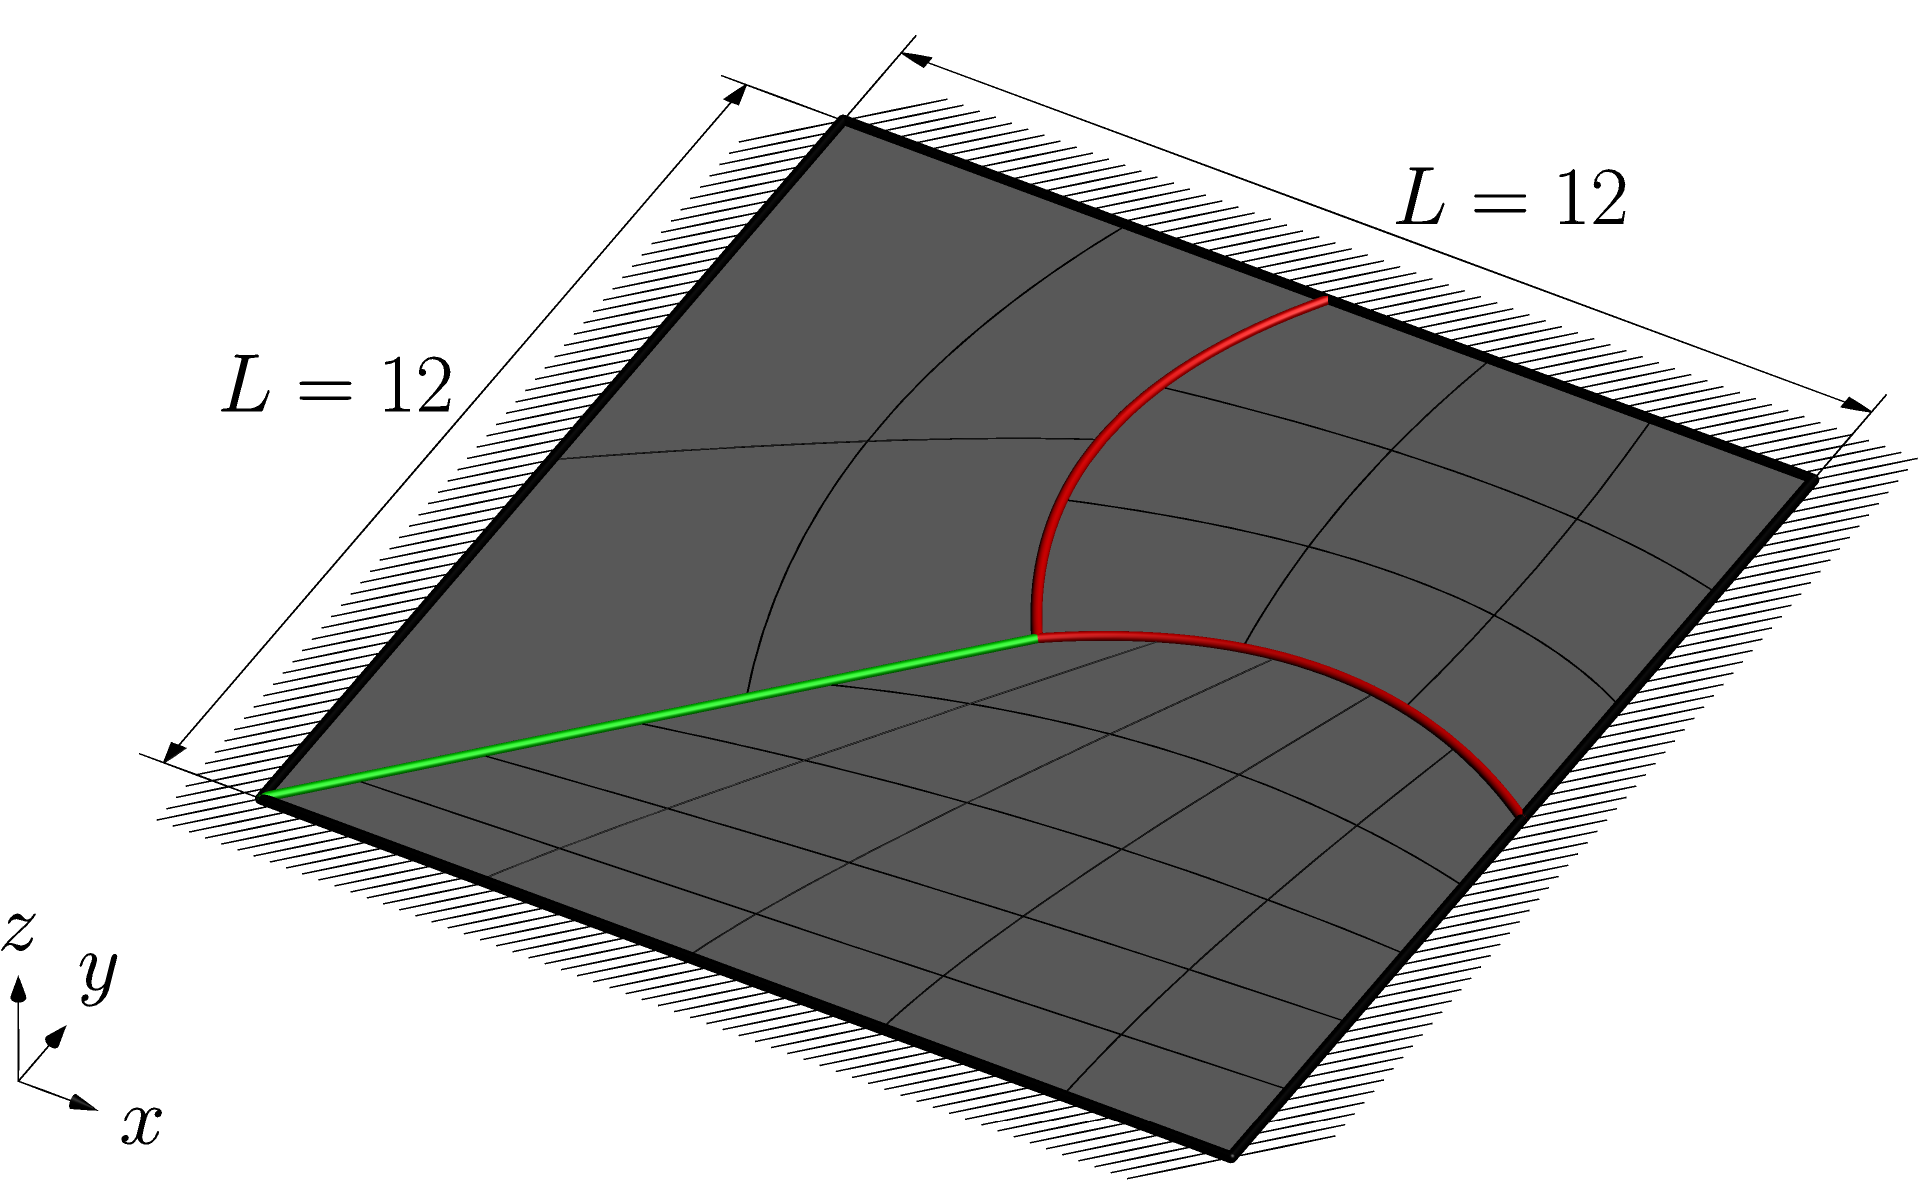
\includegraphics[scale=.4]{plate_config-plot}
		\caption{Non-matching parameterized non-conforming three-patch mesh}
	\end{subfigure}
	\begin{subfigure}[t]{.45\linewidth}
		\center
		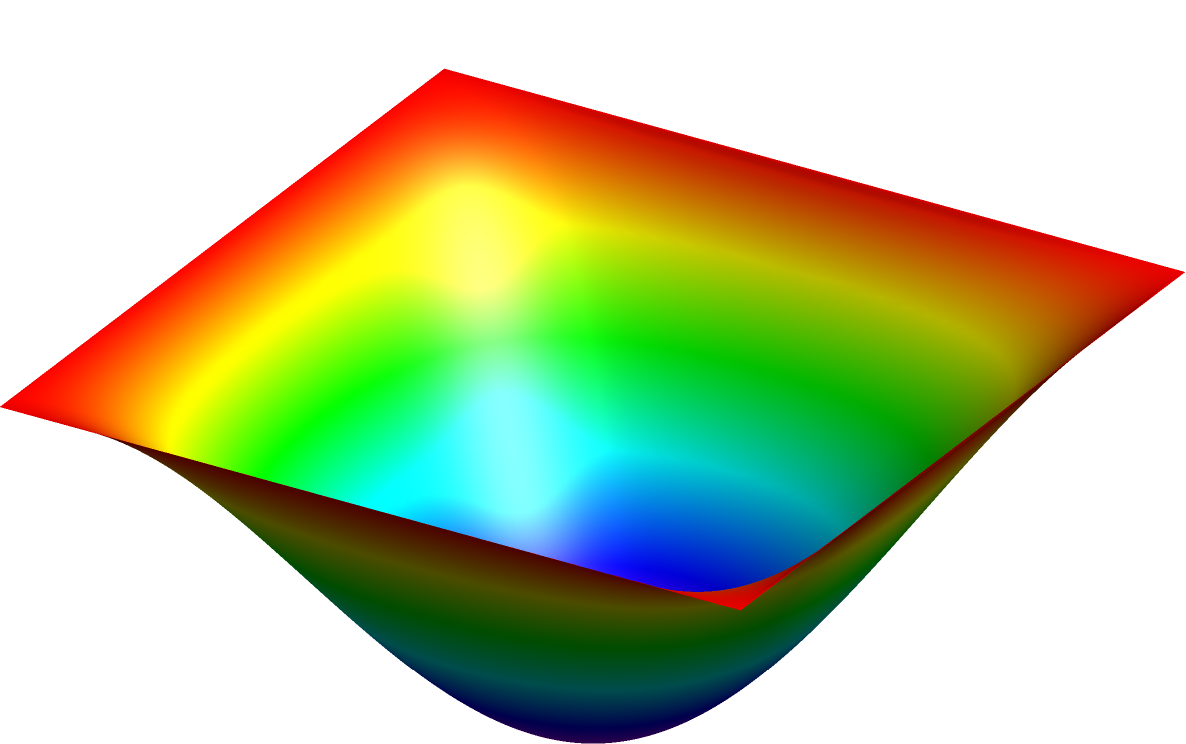
\includegraphics[scale=.3]{plate_solution-plot}
		\caption{The reference solution}
	\end{subfigure}
	\caption{The decomposition and discretization of the domain $\left[0, 1\right] \times \left[0, 1\right]$ and the refernce solution that satisfies $u=0$ on $\partial\Omega$ in Section~\ref{sec:kl-plate_problem}. The non-matching parameterized interface is denoted by green curve and the simple non-conforming discretized interfaces are denoted by red curves.}\label{fig:kirchhoff_mesh}
\end{figure}
Convergence behaviors of $w$, $M_{xx}$ and $M_{xy}$ are studied in Figure.~\ref{fig:convergence_kirchhoff}. As can be seen, both the enriched dual basis and the global dual basis yield optimal results for all polynomial orders in all three measures. As the biharmonic problem, ill-conditioning at the last refinement of $p=5$ is observed in $L^2$ norm whereas convergences of errors in $M_{xx}$ and $M_{xy}$ are still optimal. Due to the presence of a non-matching parameterized intersection, vertical shifts in error plots of the enriched dual basis have been observed for higher order elements ($p = 4,5$). Again, the \Bezier dual basis generates sub-optimal results. \par

\begin{figure}[ht]
	\center
	\captionsetup[subfigure]{labelformat=empty}
	\begin{subfigure}{.45\linewidth}
		\center
		\includestandalone[scale=.8]{three_patch_plate_L2}
	\end{subfigure}\hspace{2mm}
	\begin{subfigure}{.45\linewidth}
		\center
		\includestandalone[scale=.8]{three_patch_plate_Mx}
	\end{subfigure}\\
	\begin{subfigure}{.45\linewidth}
		\center
		\includestandalone[scale=.8]{three_patch_plate_Mxy}
	\end{subfigure}
	\caption{Convergence plots for the simply supported Kirchhoff plate in Section~\ref{sec:kl-plate_problem}. Upper left: error of $w$ measured in $L^2$ norm. Upper right: error of $M_{xx}$ measured in $L^2$ norm. Bottom: error of $M_{xy}$ measured in $L^2$ norm.}\label{fig:convergence_kirchhoff}
\end{figure}

Contour plots of $\text{err}=u_x-u_x^h$ for the simply supported Kirchhoff plate problem are given in Figure.~\ref{fig:contour_kirchhoff}. For the enriched dual basis and the global dual basis, no oscillation has been observed on the curved intersecitons, however, errors are evolved along the non-matching parameterized intersection. In addition, the influence of the non-matching intersection is more significant on the enriched dual basis case. For the case of the \Bezier dual basis, the consistency error is much higher and propagates into each patches.

\begin{figure}[ht]
	\center
	\captionsetup[subfigure]{labelformat=empty}
	\begin{subfigure}[t]{.45\linewidth}
		\center
		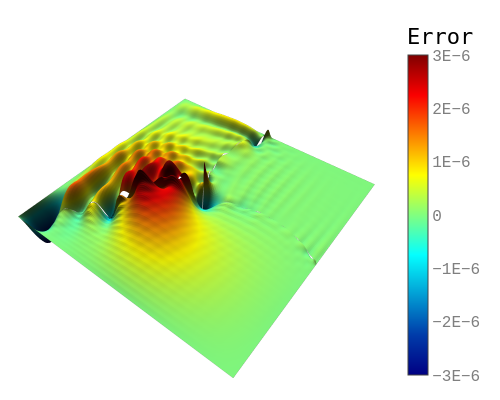
\includegraphics[scale=.4]{three_patch_plate_op_contour}
		\caption{Enrich-$Q_3$}
	\end{subfigure}
	\begin{subfigure}[t]{.45\linewidth}
		\center
		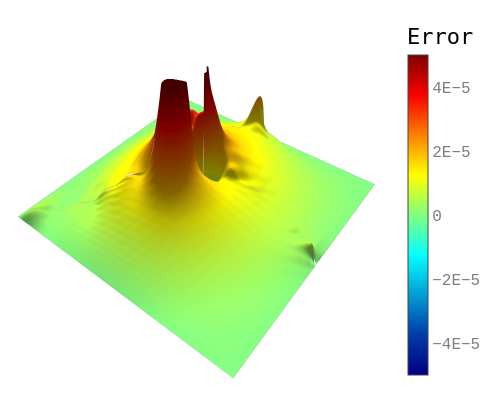
\includegraphics[scale=.4]{three_patch_plate_Bezier_contour}
		\caption{\Bezier-$Q_3$}
	\end{subfigure}\\
	\center
	\begin{subfigure}[t]{.45\linewidth}
		\center
		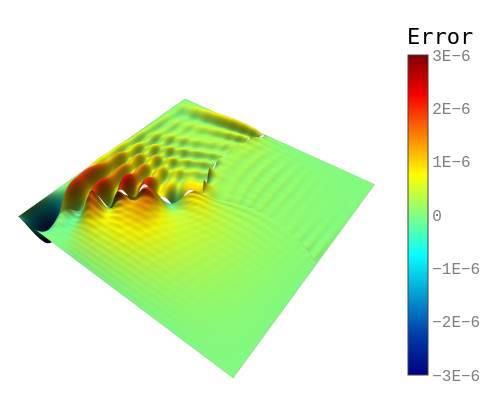
\includegraphics[scale=.4]{three_patch_plate_L2_contour}
		\caption{$L^2$-$Q_3$}
	\end{subfigure}
	\caption{Contour plots of $\text{err}=u_x-u_x^h$ for the simply supported Kirchhoff plate problem on the three-patch domain ($p=3$, and the mesh is obtained after two refinements). }\label{fig:contour_kirchhoff}
\end{figure}

\subsection{Cahn-Hilliard equation}

In this benchmark, we verify the robustness of the dual mortar method and the enriched dual basis by a $4^\text{th}$ order non-linear dynamic problem--Cahn-Hilliard equation. The Cahn-Hilliard equation is originally derived to model spinodal decomposition of binary mixtures. Taking the concentration $u$ of one of the mixtures's components as an phase-field parameter, the governing equation over infinite domain can be stated as
\begin{equation}
	\begin{split}
		\frac{\partial u}{\partial t} &= \nabla \cdot \left( M(u) \nabla\left( \mu(u)-\lambda \Delta u \right) \right)\text{ in } \Omega\times\left[ 0,T \right],\\
		u(\mathbf{x}, 0 ) &= u_0(\mathbf{x}) \text{ in } \Omega
	\end{split}
\end{equation}
where $M(u)$ is the mobility, $\mu(u)$ represents the chemical potential of a regular solution in the absence of phase interfaces and $\lambda$ is a positive constant such that $\sqrt{\lambda}$ represents a length scale of the problem. In this benchmark, we study the concentration distribution over a 2D domain with difference initial conditions and boundary conditions. We consider
\begin{align}
	M(u)   & = Du(1-u),                                                     \\
	\mu(u) & = 3\alpha\left(\frac{1}{2\theta}\log\frac{u}{1-u}+1-2u\right),
\end{align}
and adopt the following values: $\alpha=3000$, $D=1$, $\lambda = 1$ and $\theta = 1.5$. The weak form is stated as follows: find $u\in \mathcal{U}$ such that $\forall v\in \mathcal{V}$
\begin{equation}
	\langle \frac{\partial u}{\partial t}, v\rangle_\Omega + \langle M(u)\nabla \mu(u)+\nabla M(u)\Delta u,\nabla v \rangle_\Omega+\langle M(u)\Delta u,\Delta v \rangle_\Omega = 0,
\end{equation}
where $\mathcal{U}$ and $\mathcal{V}$ are suitable function spaces. \par

To achieve an optimal ratio of high-frequency and low-frequency dissipation, we adopt the first order generalized-$\alpha$ method~\cite{chung1993time, jansen2000generalized} as the temporal discretization scheme. In each time step, we require the nonlinear residual reduces to $10^{-4}$ of its initial value. For the sake of computational efficiency, we adopt an adaptive time stepping scheme introduced by G\'omez et al. in~\cite{gomez2008isogeometric}. This adaptive time stepping scheme takes advantage of the fact that the generalized-$\alpha$ method contains the backward Euler method as a special case, and use the relative error between solution from generalized-$\alpha$ method and solution from backward Euler method as an estimator of the current step size. \par

\subsubsection{Stochastic concentration distribution}

We first consider an initially stochastic concentration distribution over an infinite 2D domain, as:
\begin{equation}
	u_0(\mathbf{x}) = \bar{u}+r(\mathbf{x}),
\end{equation}
where $\bar{u}=0.63$ and the $r$ is a random variable with uniform distribution in the range $\left[ -0.005, 0.005 \right]$. The infinite domain can be described by a square domain $\Omega=\left[0 , 1\right] \times \left[0 , 1\right]$ with periodic boundary condition. Hence, for this case, both $\mathcal{U}$ and $\mathcal{V}$ are $H^2(\Omega)$ functions that satisfy periodic boundary condition. Taking into account that periodic boundary conditions are applied, it is anticipated that in the steady state only one circular inclusion remains. To demonstrate the robustness of the dual mortar method and the enriched dual basis, we non-uniformly discretize the domain $\Omega$ into $64 \times 64$ quadratic elements, the periodic boundary condition is applied by the dual mortar method.\par

The mesh and the structural evolution of the concentration distribution are demonstrated in Figure.~\ref{fig:phase_field_stochastic}. Note that both the top/bottom and the left/right interfaces are non-matching parameterized. As can be seen, from its initial stochastic pattern, the concentration distribution evolves into two phases whose composition is determined by the minima of the bulk free energy. The process is dominated by the reduction of the number of $u=0$ phase. Meanwhile, the characteristic length of $u=0$ phase is increased. Finially, the circular shape of the single inclusion is formed as the result of the bulk free energy minimization.

\begin{figure}[ht]
	\center
	\captionsetup[subfigure]{labelformat=empty}
	\begin{subfigure}[t]{.3\linewidth}
		\center
		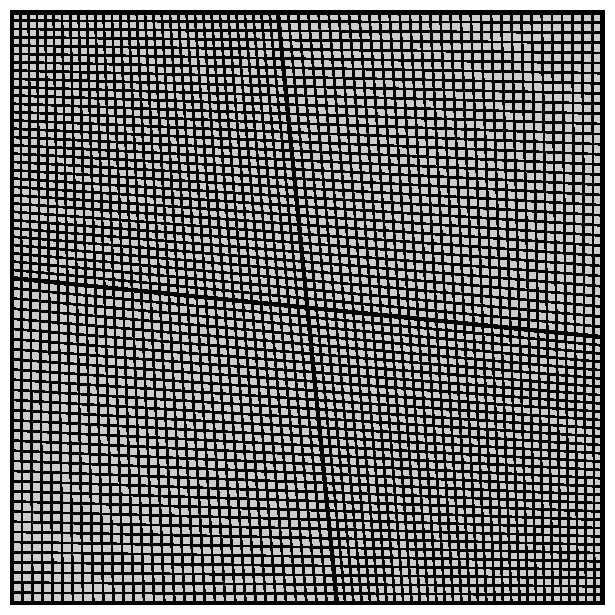
\includegraphics[scale=.431]{phase_field_domain}
		\vspace{-.4\baselineskip}
		\caption{The distorted mesh}
	\end{subfigure}
	\begin{subfigure}[t]{.3\linewidth}
		\center
		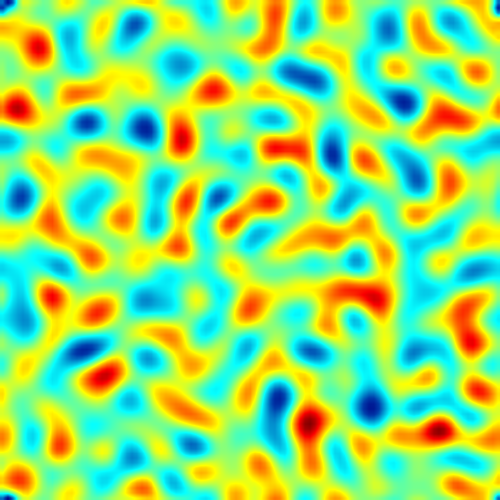
\includegraphics[scale=.25]{stochastic_ch_1_2}
		\vspace{-.4\baselineskip}
		\caption{$t=0.000002$}
	\end{subfigure}
	\begin{subfigure}[t]{.3\linewidth}
		\center
		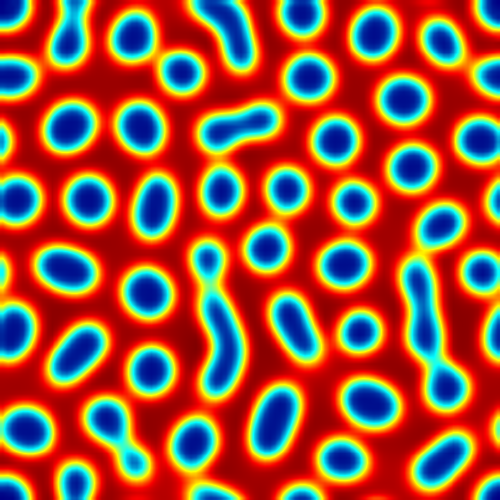
\includegraphics[scale=.25]{stochastic_ch_2_7}
		\vspace{-.4\baselineskip}
		\caption{$t=0.000007$}
	\end{subfigure}\\
	\vspace{.2\baselineskip}

	\begin{subfigure}[t]{.3\linewidth}
		\center
		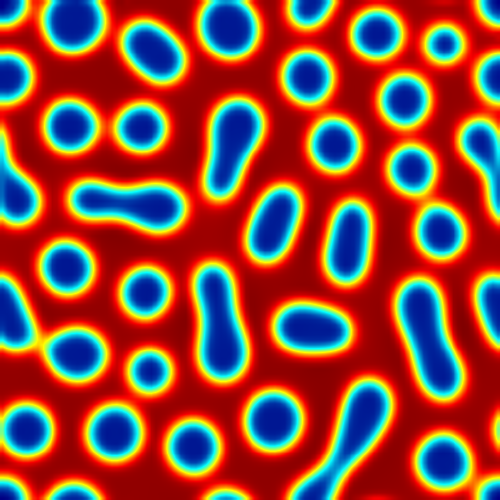
\includegraphics[scale=.25]{stochastic_ch_3_15}
		\vspace{-.4\baselineskip}
		\caption{$t=0.000015$}
	\end{subfigure}
	\begin{subfigure}[t]{.3\linewidth}
		\center
		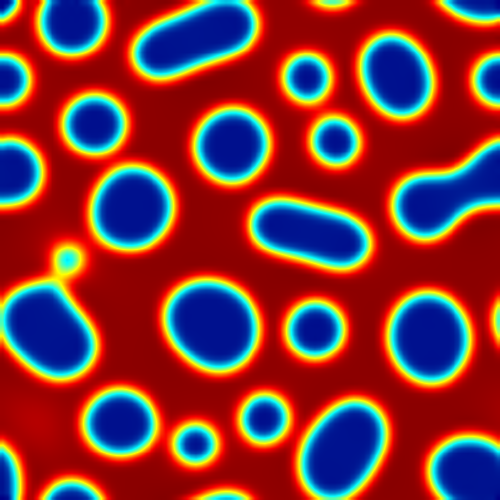
\includegraphics[scale=.25]{stochastic_ch_4_40}
		\vspace{-.4\baselineskip}
		\caption{{$t=0.000040$}}
	\end{subfigure}
	\begin{subfigure}[t]{.3\linewidth}
		\center
		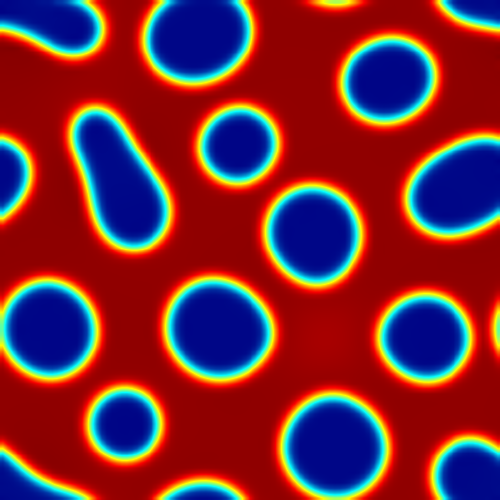
\includegraphics[scale=.25]{stochastic_ch_5_82}
		\vspace{-.4\baselineskip}
		\caption{{$t=0.000082$}}
	\end{subfigure}\\
	\vspace{.2\baselineskip}

	\begin{subfigure}[t]{.3\linewidth}
		\center
		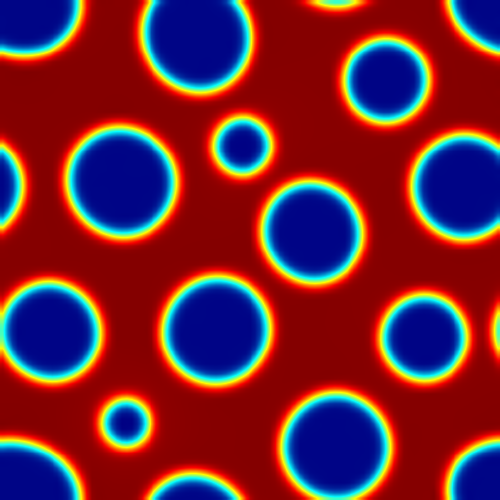
\includegraphics[scale=.25]{stochastic_ch_6_156}
		\vspace{-.4\baselineskip}
		\caption{$t=0.000156$}
	\end{subfigure}
	\begin{subfigure}[t]{.3\linewidth}
		\center
		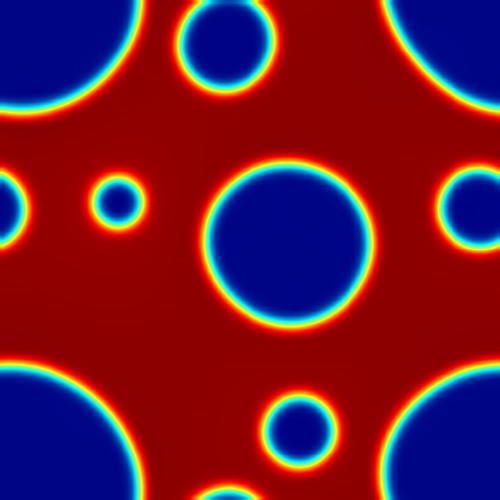
\includegraphics[scale=.25]{stochastic_ch_7_2136}
		\vspace{-.4\baselineskip}
		\caption{{$t=0.002136$}}
	\end{subfigure}
	\begin{subfigure}[t]{.3\linewidth}
		\center
		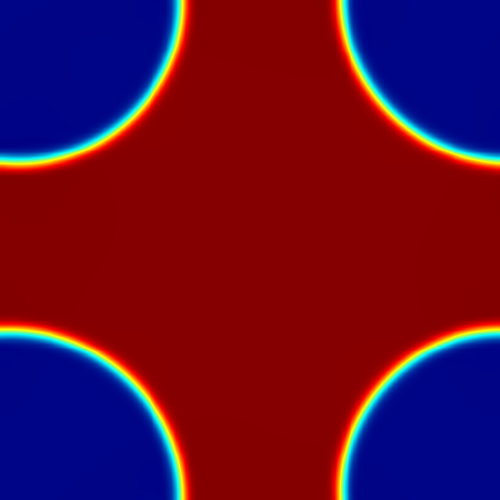
\includegraphics[scale=.25]{stochastic_ch_8}
		\vspace{-.4\baselineskip}
		\caption{Steady state}
	\end{subfigure}
	\caption{Temporal evolution of an initially stochastic concentration distribution into phases of different composition. The periodic boundary conditions are applied by the dual mortar method with the enriched dual basis. The computational domain is non-uniformly discretized, mesh lines at $\xi=0.5$ and $\eta=0.5$ are highlighted.}\label{fig:phase_field_stochastic}
\end{figure}

\subsubsection{Linear concentration distribution}

In the second case, we do not take $\bar{u}$ as a constant, but we vary it linearly with the horizontal spatial coordinate from $0.1$ to $0.9$. The domain $\Omega = \left[ 0, 2 \right] \times \left[ 0, 2 \right]$ is decomposed into four patches that are coupled non-conformingly. In addition, to show the compatibility of the coupling method with other types of boundary condition, we consider
\begin{equation}
	\frac{ \partial u}{ \partial \mathbf{n}} = 0, \;\; \text{on }\partial \Omega.
\end{equation}
This boundary condition can be incorporated into the dual mortar formulation by solving localized null space problems over each extraordinary points on the boundary. \par

The mesh and the structural evolution of the concentration distribution are demonstrated in Figure.~\ref{fig:phase_field_linear}. Four patches are discretized into $63 \times 63$, $65 \times 65$, $65 \times 65$ and $63 \times 63$ cubic elements, correspondingly. In this case, three morphologies are formed in different regions of the domain. On the left-hand side of the domain, the red phase nucleates into the blue one. The exact opposite occurs on the right-hand side. In the middle, where $u\approx 0.5$, we observe the striped pattern typical from spinodal decomposition. Whereas the nucleation process is dominated in the middle region, the structural evolution at the boundaries $x = 0$ and $x = 2$ hardly exists. Eventually, the interface develops into a straight line at $x = 1$, which is consistent with the behavior of the exact solution.\par

In both cases, the convergence of the Newton's method is achieved within $3$ interations when $\Delta t<5\times 10^{-6}$ and $4$ interations when $5\times 10^{-6} \leq \Delta t < 1\times 10^{-4}$ for both the generalized-$\alpha$ method and the backward Euler method. This is the same as the simulation with one uniformly discretized patch. In addition, no influence in the time step size of the adaptive time stepping scheme has been observed. This confirms that the dual mortar method with the enriched dual basis does not impact the convergence behavior of the correction loop and the overall performance in solving nonlinear problems.

\begin{figure}[ht]
	\center
	\captionsetup[subfigure]{labelformat=empty}
	\begin{subfigure}[t]{.3\linewidth}
		\center
		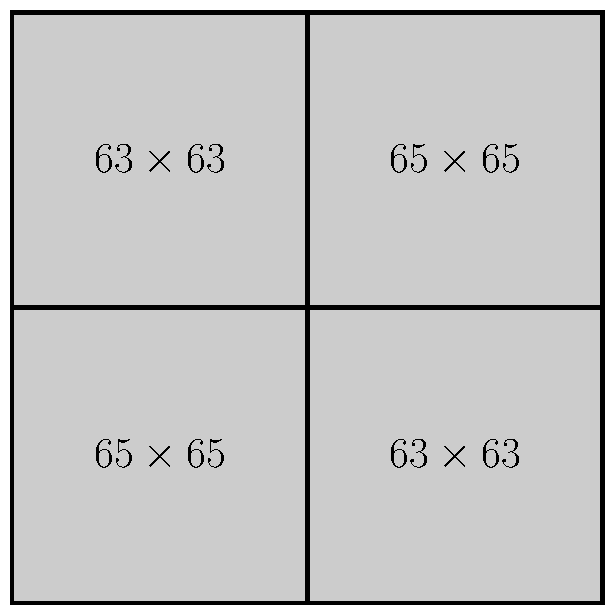
\includegraphics[scale=.431]{phase_field_domain_linear}
		\vspace{-.4\baselineskip}
		\caption{The non-conforming four-patch mesh}
	\end{subfigure}
	\begin{subfigure}[t]{.3\linewidth}
		\center
		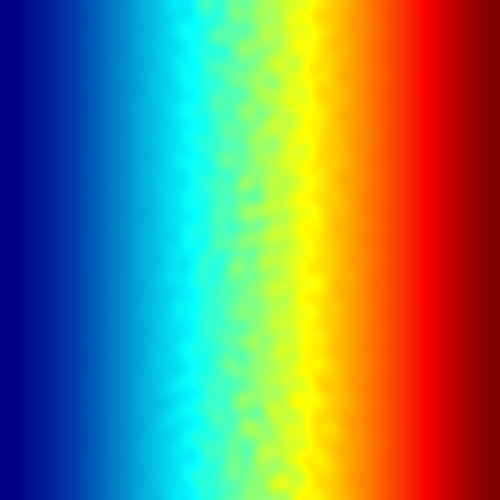
\includegraphics[scale=.25]{linear_ch_1_2}
		\vspace{-.4\baselineskip}
		\caption{$t=0.000002$}
	\end{subfigure}
	\begin{subfigure}[t]{.3\linewidth}
		\center
		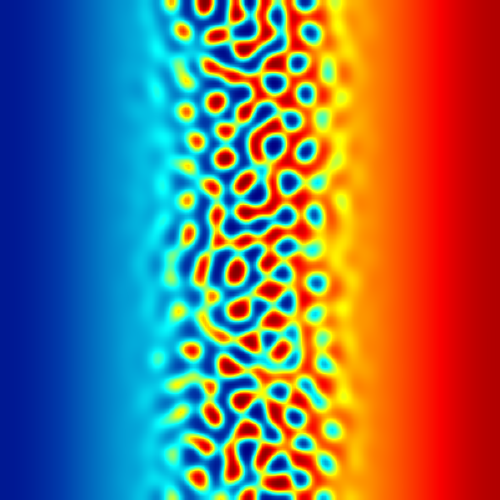
\includegraphics[scale=.25]{linear_ch_2_4}
		\vspace{-.4\baselineskip}
		\caption{$t=0.000004$}
	\end{subfigure}\\
	\vspace{.2\baselineskip}

	\begin{subfigure}[t]{.3\linewidth}
		\center
		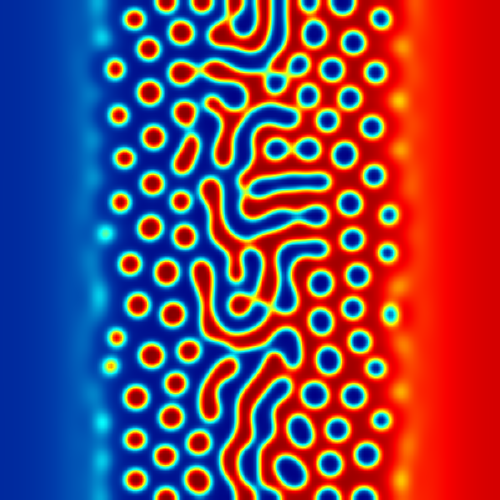
\includegraphics[scale=.25]{linear_ch_3_10}
		\vspace{-.4\baselineskip}
		\caption{$t=0.000010$}
	\end{subfigure}
	\begin{subfigure}[t]{.3\linewidth}
		\center
		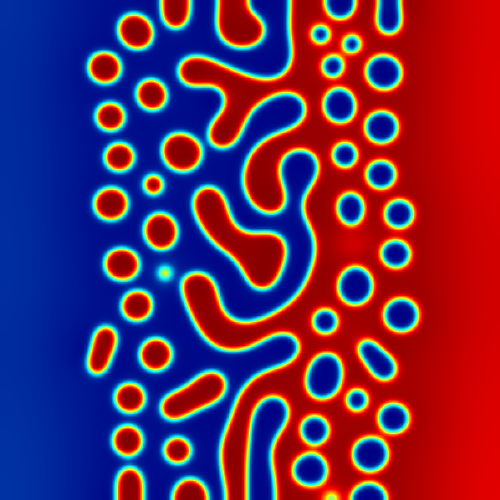
\includegraphics[scale=.25]{linear_ch_4_48}
		\vspace{-.4\baselineskip}
		\caption{{$t=0.000048$}}
	\end{subfigure}
	\begin{subfigure}[t]{.3\linewidth}
		\center
		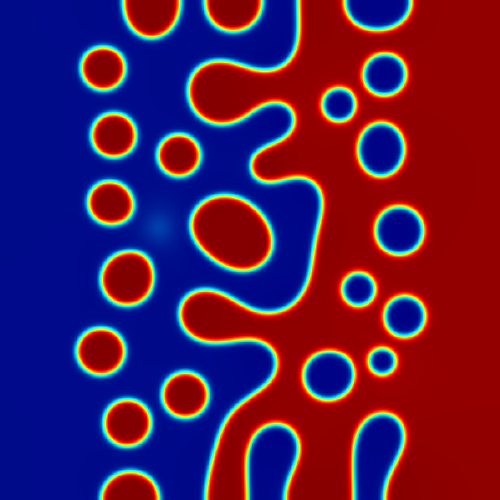
\includegraphics[scale=.25]{linear_ch_5_204}
		\vspace{-.4\baselineskip}
		\caption{{$t=0.000204$}}
	\end{subfigure}\\
	\vspace{.2\baselineskip}

	\begin{subfigure}[t]{.3\linewidth}
		\center
		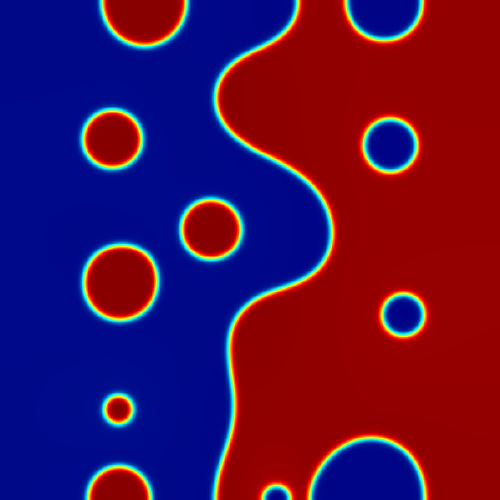
\includegraphics[scale=.25]{linear_ch_6_1304}
		\vspace{-.4\baselineskip}
		\caption{$t=0.001304$}
	\end{subfigure}
	\begin{subfigure}[t]{.3\linewidth}
		\center
		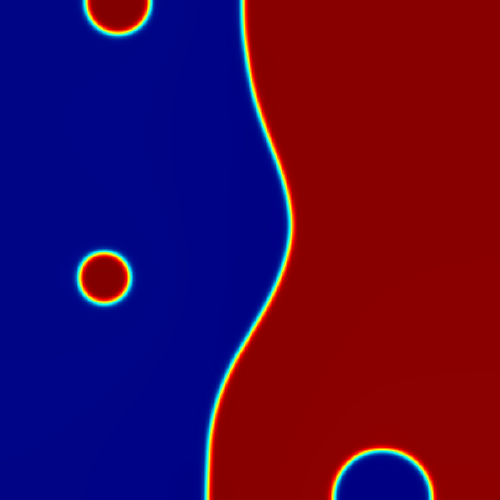
\includegraphics[scale=.25]{linear_ch_7_5814}
		\vspace{-.4\baselineskip}
		\caption{{$t=0.005814$}}
	\end{subfigure}
	\begin{subfigure}[t]{.3\linewidth}
		\center
		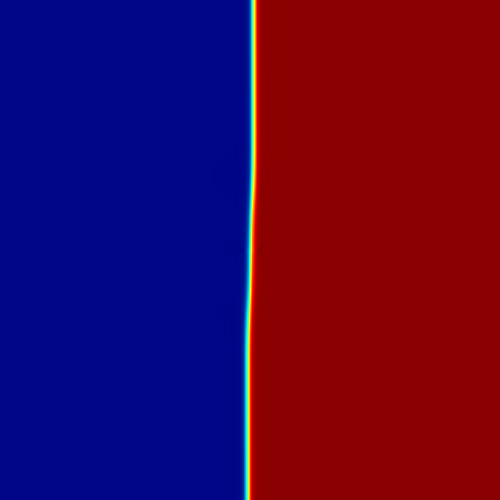
\includegraphics[scale=.25]{linear_ch_8}
		\vspace{-.4\baselineskip}
		\caption{Steady state}
	\end{subfigure}
	\caption{Temporal evolution of an initially linear concentration distribution with stochastic perturbation into two phases separated by a straight interface. The four-patch domain are coupled by the dual mortar method with the enriched dual basis.}\label{fig:phase_field_linear}
\end{figure}
\FloatBarrier

\section{Conclusion}\label{sec:conlusion}

